%; whizzy chapter
% -initex iniptex -latex platex -format platex -bibtex jbibtex -fmt fmt
% 以上 whizzytex を使用する場合の設定。

%     Tokyo Debian Meeting resources
%     Copyright (C) 2011 Junichi Uekawa
%     Copyright (C) 2011, 2013 Nobuhiro Iwamatsu
%     Copyright (C) 2012 Koichi Akabe

%     This program is free software; you can redistribute it and/or modify
%     it under the terms of the GNU General Public License as published by
%     the Free Software Foundation; either version 2 of the License, or
%     (at your option) any later version.

%     This program is distributed in the hope that it will be useful,
%     but WITHOUT ANY WARRANTY; without even the implied warranty of
%     MERCHANTABILITY or FITNESS FOR A PARTICULAR PURPOSE.  See the
%     GNU General Public License for more details.

%     You should have received a copy of the GNU General Public License
%     along with this program; if not, write to the Free Software
%     Foundation, Inc., 51 Franklin St, Fifth Floor, Boston, MA  02110-1301 USA

%  preview (shell-command (concat "evince " (replace-regexp-in-string "tex$" "pdf"(buffer-file-name)) "&"))
% 画像ファイルを処理するためにはebbを利用してboundingboxを作成。
%(shell-command "cd image201201; ebb *.png")

%%ここからヘッダ開始。

\documentclass[mingoth,a4paper,twoside]{jsarticle}
\usepackage{gum2013}
\usepackage{subfigure}
\renewcommand*\thesubfigure{}

% 日付を定義する、毎月変わります。
\newcommand{\debmtgyear}{2013}
\newcommand{\debmtgmonth}{6}
\newcommand{\debmtgdate}{29}
% (+ (* (- 2013 2005) 12) 12 -1) started from zero
\newcommand{\debmtgnumber}{95}

%% bibliography 環境を subsection に
\makeatletter%% プリアンブルで定義する場合は必須
\renewenvironment{thebibliography}[1]% 再定義
{\subsection*{\refname\@mkboth{\refname}{\refname}}%
  % \addcontentsline{toc}{section}{\refname}% この行追加
  \list{\@biblabel{\@arabic\c@enumiv}}%
        {\settowidth\labelwidth{\@biblabel{#1}}%
          \leftmargin\labelwidth
          \advance\leftmargin\labelsep
          \@openbib@code
          \usecounter{enumiv}%
          \let\p@enumiv\@empty
          \renewcommand\theenumiv{\@arabic\c@enumiv}}%
        \sloppy
        \clubpenalty4000
        \@clubpenalty\clubpenalty
        \widowpenalty4000%
        \sfcode `.\@m}
        % \setminus{.\@m}
      {\def\@noitemerr
        {\@latex@warning{Empty `thebibliography' environment}}%
        \endlist}
\makeatother%% プリアンブルで定義する場合は必須

\begin{document}

% 表紙%-------------------------------------------------------------------------
\begin{titlepage}
\thispagestyle{empty}

\hspace*{-2.5cm}

\includegraphics{image2012-natsu/gudeb.eps}\\
% % \\
% \\
%\rotatebox{10}{\fontsize{32}{32} {\gt{大統一Debian勉強会~2013~特集号}}}
\vfill
{\fontsize{30}{30}{\gt{$\sim$大統一Debian勉強会2013特集号$\sim$}}}
% \\
\vfill
% \hspace*{11cm}
\includegraphics[height=5cm]{image2013-gum/openlogo-nd.eps}\\
% \vspace*{0.1cm}
% \hfill あんどきゅめんてっど でびあん 2012年冬号 2012年12月31日 初版発行
\hfill{\fontsize{16}{16}{\gt{東京エリアDebian勉強会/関西Debian勉強会/福岡Debian勉強会\begin{flushright}-- 2013/06/29 初版発行\end{flushright}}}}
\end{titlepage}

\newpage
\thispagestyle{empty}\mbox{}
\newpage
% 表紙ここまで %---------------------------------------------------------------


% 目次 %-------------------------------------------------------------------------
\setcounter{page}{1}
\begin{minipage}[]{0.2\hsize}
 \definecolor{titleback}{gray}{0.9}
 \colorbox{dancerlightblue}{\rotatebox{90}{\fontsize{80}{80}
{\gt \color{dancerdarkblue}デビアン勉強会} }}
\end{minipage}
\begin{minipage}[]{0.8\hsize}
\hfill
\hrule
\vspace{1mm}
\hrule
\setcounter{tocdepth}{1}
{\small{\tableofcontents}}
\vspace{1mm}
\hrule
\hfill
\end{minipage}
% 目次 %-------------------------------------------------------------------------

% -------------------------------------------------------------------------
% はじめに
\dancersection{はじめに \newline $\sim$大統一Debian勉強会2013 開催概要}{「大統一Debian勉強会 2013」実行委員会}

\subsection*{開催趣意書}

Debian JP Project では2005年1月から東京地域を中心としたDebian に関する勉強会「東京エリアDebian勉強会」、
2007年3月からは関西地域を中心とした「関西エリアDebian勉強会」を毎月、2013年1月からは九州福岡地域で「福岡Debian勉強会」を行なっています。


\vspace{1zw}
Debian 勉強会の大きな目的として、
\begin{itemize}
\item Debian Developer の育成
\item 普段全国各地にいる人々が face-to-face で出会える場を提供する
\end{itemize}
があります。

\vspace{1zw}
昨年(2012年)、
各地のDebian勉強会が京都に集結し、Debianユーザ、Debian開発者の交流を目的とする「大統一Debian勉強会」
を開催し大盛況に終わりました。今年は場所を東京に移し、大統一Debian勉強会 2013を開催します。

\vspace{1zw}
2013年度の本イベントのテーマは
\begin{center}
  {\bf{「Level up Debian」}}
\end{center}
です。

\vspace{1zw}
今回のイベントに参加することによって、Debianの新しい使い方を知り、一歩進んだ活用ができるようになることを考えています。

\vspace{1zw}
2012年に開催した大統一Debian勉強会の成功を受け、よりよいイベントの開催と世界各国で毎年開催されている DebConf(Debian カンファレンス)\footnote{\url{http://debconf.org/}}を日本で開催することを目指しています。

\pagebreak

\subsection*{本資料に関して}

会場で頒布される本資料は大統一 Debian 勉強会 2013 のスポンサーのご支援に
より、出版できました。スポンサーの皆様に感謝します。ありがとうございまし
た。

\subsubsection*{スポンサー一覧(敬称略)}

\begin{itemize}
\item プラチナスポンサー
  \begin{itemize}
  \item 株式会社マイクロソフト
  \end{itemize}
\item ゴールドスポンサー
  \begin{itemize}
  \item ぷらっとホーム株式会社
  \item 株式会社トップスタジオ
  \item 株式会社サーバーワークス
  \end{itemize}
\item シルバースポンサー
  \begin{itemize}
  \item ミラクル・リナックス株式会社
  \item 株式会社サイバーエージェント
  \item さくらインターネット株式会社
  \end{itemize}
\item メディアスポンサー
  \begin{itemize}
  \item アイティメディア株式会社
  \item 株式会社技術評論社
  \item gihyo.jp
  \item sourceforge.jp
  \item 株式会社アスキー・メディアワークス
  \end{itemize}
\item ウェブサイトスポンサー
  \begin{itemize}
  \item ANNAI LLC
  \end{itemize}
\item 協賛
  \begin{itemize}
  \item 会場提供: 日本大学
  \item ペットボトル(ミネラルウォーター) 提供:株式会社サイバーエージェント
  \end{itemize}
\end{itemize}


\pagebreak
% -------------------------------------------------------------------------
% 岩松さん
\dancersection{debhelper におけるプログラミング言語ビルドツール対応の仕組みについて}{岩松 信洋}
\label{sec:debhelper}

Debian は多くのプログラミング言語をサポートしており、それらを使ったソフトウェアが多く存在します。
Debian の各プログラミング言語サポートチームはパッケージのメンテナンスを軽減するために パッケージ
作成サポートツールの一つである debhelper 向けツールを作成し、提供しています。
一部で流行っているプログラミング言語 Erlang ですが、もちろん Debianでもサポートされています。
最近の Erlang アプリケーションのほとんどは rebar というビルドサポートツールを使ってビルドされますが、
まだrebarをサポートした debhelper 向けツールがありません。よって rebar を使っているアプリケーションを
Debianパッケージにする場合には必要な処理を debian/rules に記述する必要があります。
私は rebar と rebar を使った Erlang アプリケーションパッケージをメンテナンスしています。
今回 rebar を使った Erlang プログラムを他のプログラミング言語同様に、容易にDebianでサポートできるように、
rebar の debhelper 実装\texttt{dh-rebar}を開発することにしました。
本章ではこのツール \texttt{dh-rebar} についての解説とdebhelper におけるプログラミング言語対応の仕組みについて説明
します。

\subsection{rebar とは}

まず、rebar の仕組みについて簡単に説明します。
reabr はプログラミング言語 Erlang のビルドツールです。Riak の開発元として有名な
Basho\footnote{\url{http://basho.com/}} によって開発が
行われています。rebar は Erlang を使ったビルドやテスト、ドキュメント作成からプロジェクトのひな形作成まで
サポートしており、今では多くの Erlang アプリケーションで利用されています。
rebar によって提供されている主要なコマンドを以下に示します。

\begin{itemize}
\item rebar compile : Erlang プログラムをコンパイルする。
\item rebar clean : コンパイル時に作成された一時ファイルの削除する。
\item rebar eunit : テストを実行する。
\item rebar doc : ドキュメントの作成する。
\item rebar xref : モジュールや関数の依存関係のチェックを行う。
\item rebar get-deps : ビルドに必要なライブラリなどのソースコードを取得し、コンパイルする。
\end{itemize}

これらのコマンドは単体で呼ぶこともできますが、多くの場合ソースコードにMakefileが含まれており、
Makefileから rebar の各コマンドが利用する形になっています。
またインストールに関する処理は用意されておらず、ビルドされたものをそのまま参照するか、ユーザが
インストール処理を行う必要があります。図\ref{fig:debhelper-makefile}に Makefile の例を示します。

\begin{figure}[h!]
\centering
\begin{commandline}
(省略)
deps:
    @./rebar get-deps

app:
    @./rebar compile
(省略)
\end{commandline}
\caption{Makefile 例}\label{fig:debhelper-makefile}
\vspace{-1.5em}
\end{figure}

Makefileの例を見てもわかるように、rebar は相対パスで指定されていることが多く、rebar のバイナリをソースコードに
含めるている事がほとんどです。
この理由として、過去に rebar の仕様が頻繁に変更されたことがあり、そのたびにビルドできないという問題があったようです。
その対策のためにソースコードにrebarバイナリを含めるようになったとのことです。
そのため、Debianパッケージにする場合にはソースコードから rebar バイナリを削除する作業が必要となります。

\subsubsection{rebar を使ったDebianパッケージ の作業}

上記のようなビルドシステムである rebar を使っているソフトウェアを Debian パッケージにする場合、
主に以下のような作業が必要になります。

\begin{enumerate}
\item %
  rebar バイナリをソースから削除し、ソースコードをリパックする。パッケージのバージョンに+dfsg をつける。
  \texttt{debian/README.source}にこれについて記載する。

\item %
  dh\_make を実行して雛形を作成する。

\item %
  override\_dh\_auto\_build build が呼ばれた時には rebar compile、
  override\_dh\_auto\_test が呼ばれた時に rebar test、
  override\_dh\_auto\_clean が呼ばれた時に rebar clean 実行するなどの処理を debian/rules に追加する。

\item %
  DebianのErlang パッケージはプレフィックスにerlang- をつける。

\item %
  作成されたバイナリをusr/lib/erlang/lib/\$(PACKAGE)-\$(VERSION)/以下にインストールされるように処理する。\\
  PACKAGE には元のパッケージ名、VERSION には元のパッケージのバージョン
  が指定される。例えば erlang-foo の Debian バージョン 1.0.0+dfsg-1 の場合は
  PACKGE に foo、VERSION には 1.0.0 が入る。
\item %
  .beam と .erl は 圧縮されないように dh\_compress で無視するように設定する。
\end{enumerate}
% $

上記の作業を行った後の \texttt{debian/rules} は図\ref{fig:debhelper-debianrules}のようになります。
%
\begin{figure}[ht]
  \centering
\begin{commandline}
#!/usr/bin/make -f

PACKAGE = $(shell dpkg-parsechangelog | sed -rne 's/^Source: erlang-(.*)/\1/p')
VERSION = $(shell dpkg-parsechangelog | sed -rne 's/^Version: ([0-9.]+)(\+dfsg)?.*$$/\1/p')

%:
    dh $@

override_dh_auto_build:
    rebar compile -vv skip_deps=true

override_dh_auto_clean:
    dh_auto_clean
    rm -rf ebin

override_dh_auto_install:
    dh_auto_install

    install -d \
        $(CURDIR)/debian/erlang-$(PACKAGE)/usr/lib/erlang/lib/$(PACKAGE)-$(VERSION)/ebin
    install -m 644 ebin/* \
        $(CURDIR)/debian/erlang-$(PACKAGE)/usr/lib/erlang/lib/$(PACKAGE)-$(VERSION)/ebin/
    install -d \
        $(CURDIR)/debian/erlang-$(PACKAGE)-dev/usr/lib/erlang/lib/$(PACKAGE)-$(VERSION)/include
    install -m 644 include/* \
        $(CURDIR)/debian/erlang-$(PACKAGE)-dev/usr/lib/erlang/lib/$(PACKAGE)-$(VERSION)/include/

override_dh_gencontrol-arch:
    erlang-depends -v -a -perlang-$(PACKAGE)
    erlang-depends -v -a -perlang-$(PACKAGE)-dev
    dh_gencontrol -a -perlang-$(PACKAGE)
    dh_gencontrol -a -perlang-$(PACKAGE)-dev

override_dh_compress:
    dh_compress -X.erl -X.beam
\end{commandline} %$
 \caption{debian/rules 例}
 \label{fig:debhelper-debianrules}
 \vspace{-1.5em}
\end{figure}

Debian パッケージビルドサポートツールの一つである debhelperのバージョン7(以下、debhelper7)
の機能を使っているにも関わらず、35行と比較的長い\texttt{debian/rules}になっています。
ざっと見てみると、共通化できる部分がいくつかありそうです。共通化できる部分をまとめると
もっと短い \texttt{debian/rules} になりますし、コーディングミスも減ることが考えられます。
また、仕様変更や問題があった場合にも 共通部分を修正するだけで対応できるようになります。
そこで共通部分を debhelper の機能 \texttt{dh-rebar} として提供することにしました。
次に debhelper による rebar を使った Erlang プログラムのサポートについて説明します。

\subsection{debhelper によるプログラミング言語のサポート}

debhelper7 からビルドシステムを追加する機能 Buildsystem とビルドシーケンスをコントロールする機能
Sequence が追加されました。
%debhelper 7 より前はこのような機能がなかったため、CDBS と呼ばれる別の
%パッケージビルドサポートツールが使われることが多かったのですが、現在は立場は逆転しています。
これらの機能には、オーバライドできる機能もあるため、これを使うことによって容易にプログラミング言語や
ツールのサポートができるようにもなっています。
Buildsystem と Sequence の概要と rebar での実装方法について実際のコードを使って説明します。

\subsubsection{Buildsystem / ビルドシステム}

Buildsystem では \texttt{clean}、\texttt{configure}、 \texttt{build}、\texttt{install}、
\texttt{test} 関数が提供され、デフォルトではシンプルな Makefileをターゲットにした処理が
行われるようになっています。
これらの関数はオーバーライドすることができ、各々に必要な処理を新しい Buildsystem として記述すること
によって、プログラミング言語などをサポートできるようになってます。
記述した Buildsystem を\texttt{/usr/share/perl5/Debian/Debhelper/Buildsystem/}
にインストールし、dhコマンド(debhelper) の \texttt{--buildsystem} オプションで指定
することによってパッケージビルド時に利用されるようになります。
利用できる Buildsystem は \texttt{dh\_auto\_build} の \texttt{--list} オプションで確認できます
(図\ref{fig:debhelper-dhautobuild})。

\begin{figure}[ht]
  \centering
\begin{commandline}
$ dh_auto_build --list
perl_makemaker       Perl ExtUtils::MakeMaker (Makefile.PL)
makefile             simple Makefile
rebar                rebar [3rd party]

Auto-selected: makefile
\end{commandline} %$
 \caption{\texttt{dh\_auto\_build --list} 出力例}
 \label{fig:debhelper-dhautobuild}
 \vspace{-1.5em}
\end{figure}

次に、Buildsystem で提供される関数をオーバーライドする例を図\ref{fig:debhelper-buildsystem}に示します。
例ではbuild 関数をオーバーライドし、\$DH\_REBAR\_MAKEFILE で指定されている dh-rebar.Makefile
の build ターゲットが実行されるようになっています。
これにより、debian/rules から build ターゲットが呼ばれた時に、新しく作成した rebar Buildsystem
の build 関数が呼ばれるようになります。

\begin{figure}[ht]
  \centering
\begin{commandline}
package Debian::Debhelper::Buildsystem::rebar;

use strict;
use base 'Debian::Debhelper::Buildsystem';

my $DH_REBAR_MAKEFILE="/usr/share/dh-rebar/make/dh-rebar.Makefile";

sub DESCRIPTION { "rebar" }

(省略)

sub build {
    my $this=shift;
    $this->doit_in_sourcedir("make", "--no-print-directory", "-f", $DH_REBAR_MAKEFILE, "build", @_);
}

(省略)
\end{commandline}
%$$
 \caption{Buildsystem オーバライド例}
 \label{fig:debhelper-buildsystem}
 \vspace{-1.5em}
\end{figure}

次にBuildsystem から実行される dh-rebar.Makefile について説明します。
内容の一部を図\ref{fig:debhelper-dhrebarmakefile}に示します。

\begin{figure}[h!]
\centering
\begin{commandline}
(省略)
include debian/dh-rebar.conf
(省略)
# build
ifneq (,$(findstring xref, $(EXEC_REBAR_COMMANDS)))
BUILD_TARGET+=rebar_xref
endif
ifneq (,$(findstring compile, $(EXEC_REBAR_COMMANDS)))
BUILD_TARGET=rebar_compile
endif

build: $(BUILD_TARGET)

rebar_compile:
    $(H)echo $@
    rebar compile skip_deps=true -v

rebar_xref:
    $(H)echo $@
    rebar xref skip_deps=true -v
(省略)
\end{commandline}
%$
 \caption{dh-rebar.Makefile}
 \label{fig:debhelper-dhrebarmakefile}
\begin{commandline}
EXEC_REBAR_COMMANDS=compile
PKG_NAME=
PKG_VARSION=
#REBAR_LIB_DIR=
#REBAR_BIN_DIR=
#REBAR_INCLUDE_DIR=
\end{commandline}
 \caption{dh-rebar.conf 例}
 \label{fig:debhelper-dhrebarconf}
\end{figure}

dh-rebar.Makefile では build ターゲットが呼ばれた時に\$(BUILD\_TARGET)が実行されるようになっており、
\$(EXEC\_REBAR\_COMMANDS) の内容によって変化します。
\$(EXEC\_REBAR\_COMMANDS) に compile がある場合は BUILD\_TARGET に rebar\_compile
が追加され、\$(EXEC\_REBAR\_COMMANDS) に xref がある場合は BUILD\_TARGET
に rebar\_xref が追加されます。
そして rebar\_compileでは \texttt{rebar} の compile、rebar\_xref では  xref が実行される
ようになっています。
\$(EXEC\_REBAR\_COMMANDS) などの変数は debian ディレクトリにある\texttt{dh-rebar.conf}
(図\ref{fig:debhelper-dhrebarconf})を参照するようになっています。
このファイルによって、実行される Makefile のターゲットやバイナリがインストールされる参照先
や、実行するMakefileのターゲットをコントロールできるようになっています。

rebar の場合は、ソフトウェアのビルドやテストがコマンド毎に決まっているので
その動作に合わせて dh-rebar.Makefile を記述しました。
Buildsystemからは 図\ref{fig:debhelper-image01}のような流れでビルドを行うようになっています。

\begin{figure}[h!]
  \centering
  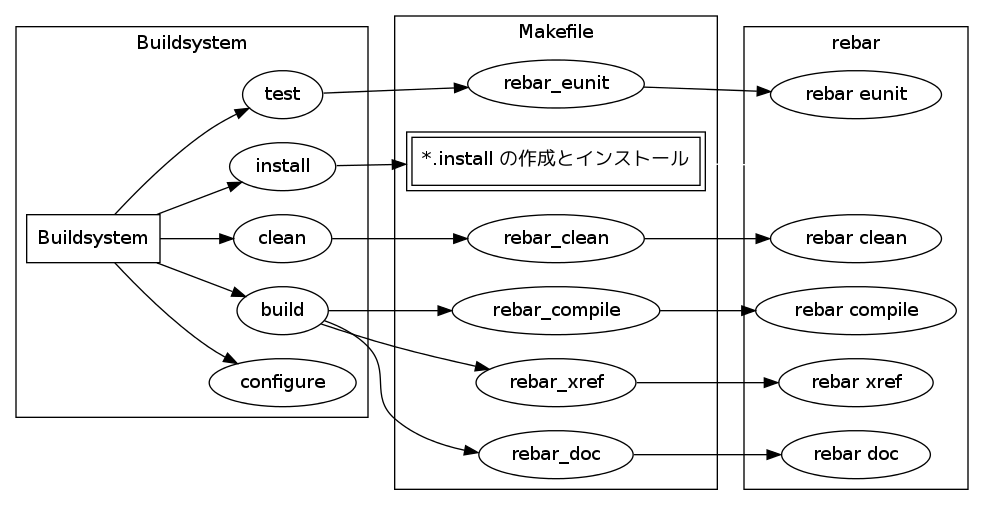
\includegraphics[width=0.7\hsize]{image2013-gum/buildsystem.png}
  \caption{全体の流れ}
  \label{fig:debhelper-image01}
  \vspace{-1.5em}
\end{figure}

また、今回は Buildsystem から Makefile を呼ぶようにしましたが、代わりにシェルやpythonなどのスクリプトで
実装してもかまいません。

\subsubsection{Sequence / シーケンス}

Sequence は dh 内で実行される dh コマンド群のパッケージビルドシーケンスをコントロールします。
dh では実行されるパッケージビルドシーケンスとして、決まったシーケンスを持っており何もしない場合には
この決まったシーケンスが実行されます。Sequence 機能を使うと、ある dh コマンドを実行しないよう抑制したり、
ある dh コマンドの前後に独自の処理を挿入できるようになります。

Erlang の場合はソースコードやバイナリのサフィックスに\texttt{.erl}や\texttt{.beam}
が付与されているのですが、これらのファイルをパッケージにする場合に圧縮させたくありません。
圧縮すると Erlang のプログラムとして利用できないためです。
よって Erlang パッケージの場合は 必ず \texttt{dh\_compress} (パッケージ内のファイルを圧縮するコマンド)
を実行する時にこれらのファイルを無視するように設定します。
これには \texttt{add\_command\_options} を使って、\texttt{dh\_compress} にオプションを設定します。

\begin{commandline}
add_command_options("dh_compress", "-X.erl -X.beam");
\end{commandline}

また、ある debhelper コマンドの前後に別のdebhelper のコマンドを実行させたい場合があります。
この場合 \texttt{insert\_before}または\texttt{insert\_after}を使って、実行したい
コマンドを指定します。

Erlang パッケージ間の依存関係をチェックし、バイナリパッケージの control ファイルに記述するツール \texttt{erlang-depends}
があるのですが、これを \texttt{dh\_gencontrol}\footnote{debian/controlを変換しインストールする debhelper ツールの一つ}
の前に呼ぶ必要があります。erlang-depends は debhelper7 に対応していないので、ラッパーした\texttt{dh\_rebar} を作成し、
以下のように記述しました。

\begin{commandline}
insert_before("dh_gencontrol", "dh_rebar");
\end{commandline}

このような設定を記述したファイル(図\ref{fig:debhelper-sequence})を rebar.pm として、\texttt{usr/share/perl5/Debian/Debhelper/Sequence/}
にインストールします。そして dh のオプション \texttt{--with} で指定することによりファイル内
で指定したシーケンスがパッケージビルド時に有効になります。

\vspace{-1em}
\begin{figure}[h!]
  \centering
\begin{commandline}
#! /usr/bin/perl

use warnings;
use strict;
use Debian::Debhelper::Dh_Lib;

insert_before("dh_gencontrol", "dh_rebar");

add_command_options("dh_compress", "-X.erl -X.beam");

1;
\end{commandline}
\caption{Sequence ファイル}
\label{fig:debhelper-sequence}
\end{figure}
\vspace{-2.5em}

\subsection{dh-rebar を使った debian/rules}

上記で説明した dh-rebar で提供される Buildsytem と Sequence を使って
debian/rules を書きなおすと、以下のようになります。
35行が3行になり、シンプルになりました。また、各種設定は \texttt{debian/dh-rebar.conf}
にまとめられるため、debian/rules も特に編集する必要はなくなります。

\begin{commandline}
#!/usr/bin/make -f
%:
    dh $@ --buildsystem=rebar --with rebar
\end{commandline}
%$

\subsection{まとめ}

debhelper7 から提供されている Buildsystem と Sequence を使うと、Debian パッケージにする時に
必要な機能をまとめることができます。また、まとめられた機能を使うことによって容易にパッケージに
できるようになり、メンテナンス性もよくなります。
今後新しいプログラミング言語やビルドツールをサポートするときの手助けになれば幸いです。

\pagebreak
%-------------------------------------------------------------------------
% 野島さん
\dancersection{gdb+python拡張を使ったデバッグ手法}{野島 貴英}
\label{sec:gdb-python-php}

debian付属のgdbはすでにpython拡張が有効になっている状態でパッケージ化されています。
今回の発表では、debianに用意されている機能をフル活用して、PHP5のPHP言語レベルの
ソースデバッグをgdb+pythonをつかってやってみる事について述べます。

なお、ここでは、debian sid(jessie/sid)を用い、パッケージから導入したgdb 7.6、PHP 5.5.0rc3を利用しています。

\subsection{gdb+python拡張今までのおさらい}

gdbは、バイナリ形式の実行ファイルをデバッグするのに、極めて強力な
シンボリックデバッガです。gdbはpythonを内臓することにより、さらに強力なデバッグが可能になっています。debianではsqueezeから有効になっています。

東京エリアdebian勉強会の2013年3月にては、gdb+python拡張に搭載されているgdb.Command/ gdb.Breakpoint/ gdb.FinishBreakpointを使い、C言語による実行ファイルの関数トレースを取るところまで紹介しました\cite{tokyo-debian-march}。

\subsection{debianの*-dbgパッケージについてちょっとだけ}

debianには、バイナリパッケージのデバッグ用シンボル情報だけを集めた
*-dbgパッケージ群が提供されています。
%
利用の仕方は簡単で、デバッグしたいバイナリパッケージの名前に-dbgと付いた
パッケージを導入し、gdbを動かすだけです。

\begin{commandline}
% sudo aptitude install 'php5-dbg'
% apt-get source php5
% gdb --args /usr/bin/php5 -r 'phpinfo();'
...中略...
(gdb) b main
Breakpoint 1 at 0x4640a0: file /tmp/buildd/php5-5.5.0~rc3+dfsg/sapi/cli/php_cli.c, line 1200.
(gdb) set substitute-path /tmp/buildd/ ./
(gdb) run
Starting program: /usr/bin/php5 -r phpinfo\(\)\;
...中略...
Breakpoint 1, main (argc=3, argv=0x7fffffffe668)
    at /tmp/buildd/php5-5.5.0~rc3+dfsg/sapi/cli/php_cli.c:1200
1200	{
(gdb) l (←現在実行中のソースコードを閲覧)
1195	#ifdef PHP_CLI_WIN32_NO_CONSOLE
1196	int WINAPI WinMain(HINSTANCE hInstance, HINSTANCE hPrevInstance, LPSTR lpCmdLine, int nShowCmd)
1197	#else
1198	int main(int argc, char *argv[])
1199	#endif
1200	{
1201	#ifdef ZTS
...中略...
\end{commandline}

(なお、上の例ではソースコード指定に ''set substitution-path'' を利用しましたが、
現状では必ずしもこれでうまく行くものばかりではない事を後に述べます。)

なお、*-dbgパッケージに関しての現状と詳細は2012年の大統一Debian勉強会の岩松さんの発表"debug.debian.net"\cite{debug-debian-net}に詳しいです。ここでは、そこで触れられていなかった件をいくつか載せておきます。

\subsubsection{ソースコードのパスの指定について}

*-dbgパッケージを利用してgdbからソースコードを指定するための指定方法は、
以下の2種類の方法を適宜選んで指定します。

\begin{itemize}
\item gdbの ``set substitute-path'' で指定する方法\\
  これは、パッケージがビルドされる際、gccに対してソースがフルパスで指定されているときに使える方法となります。先ほどのPHP5の例のように、
  一つの''set substitute-path''を指定するだけで、ソースのサブディレクトリに配置されているソースコードも正確に自動でgdbが追跡してくれますので、デバッグ時のソース閲覧に大変都合が良いです。
\item gdbの ``dir'' でソースの位置を複数指定する方法\\
  これは、パッケージがビルドされる際、gccに対してファイル名のみ指定されてコンパイルされている場合に使います。こちらの場合、*-dbgパッケージのシンボルにソースのパスを示す情報が欠落している為、ソースの位置は''dir''コマンドでヒントとして指定することになります。gdbはユーザが''dir''コマンドで指定したソースの存在するパス全部を記憶しており、このパスに同名のファイルがあるかを調べ、最初に合致したものを表示します。つまり、完全に同名のファイルが複数のサブディレクトリに配置されていたものをビルド及びリンクした場合は、gdbは自動では正しいソースファイル上での位置を表示できない為、注意が必要です。
\end{itemize}

\subsubsection{debhelperのCOMPATIBILITY LEVEL 9から搭載されたデバッグシンボルファイルの形式について}

パッケージ構築の際、debhelperのCOMPATIBILITY LEVEL 9から、導入されたデバッグ用シンボルファイルのファイル名は、パッケージの実行ファイルのバイナリに埋め込まれているBuildID
\cite{build-id-desc}というハッシュ値を元につけられています。以前の形式では、実行バイナリの名前がそのままデバッグ用シンボルファイルとなっていました。

\begin{commandline}
#↓ COMPATIBILITY LEVEL 9形式の場合
$ file /usr/lib/x86_64-linux-gnu/libgstreamer-0.10.so.0.30.0
/usr/lib/x86_64-linux-gnu/libgstreamer-0.10.so.0.30.0: ELF 64-bit LSB
shared object, x86-64, version 1 (SYSV), dynamically linked,
BuildID[sha1]=44ff321f11ffd750f8c351ffa3f5d20028d2f6a6, stripped
# 表示されたBuildIDの、上2桁及び残りの桁をもちいて
# /usr/lib/debug/.build-id/上2桁/残りの桁.debugとなるファイルが
#デバッグ用シンボルファイルとなる。
$ ls /usr/lib/debug/.build-id/44/ff321f11ffd750f8c351ffa3f5d20028d2f6a6.debug
/usr/lib/debug/.build-id/44/ff321f11ffd750f8c351ffa3f5d20028d2f6a6.debug
# 試しにCOMPATIBILITY LEVEL 9形式で作成されたバイナリをgdbでロードしてみる
# gdb起動メッセージに含まれるReading symbols from 以下のファイル名のとおり、
# BuildIDで決まるシンボルファイルを読みにいく。
$ gdb /usr/lib/x86_64-linux-gnu/libgstreamer-0.10.so.0.30.0
GNU gdb (GDB) 7.6-debian
...中略...
Reading symbols from /usr/lib/x86_64-linux-gnu/libgstreamer-0.10.so.0.30.0...
Reading symbols from /usr/lib/debug/.build-id/44/ff321f11ffd750f8c351ffa3f5
d20028d2f6a6.debug...done.
(gdb) quit
#↓ COMPATIBILITY LEVEL 9形式未満の場合
# シンボルファイルは"/usr/lib/debug/"+"デバッグ対象の実行ファイルの絶対パス名"に格納
$ ls -l /usr/lib/debug/usr/bin/php5
-rw-r--r-- 1 root root 22036903  6月  2 01:44 /usr/lib/debug/usr/bin/php5
\end{commandline}

gdbのようなデバッグ用シンボルファイルを扱うソフトウェアとしては、バイナリのBuildIDさえ分かれば、正しいデバッグ用シンボルファイルをすぐに特定できるので都合がよかったりします。従来のように同じファイル名のデバッグ用シンボルファイルを用意するという方法の場合、正しいデバッグ用シンボルファイルであることを保証するには、わざわざシンボルファイルのチェックサムを取って確認するぐらいしかありませんでした\cite{build-id-desc}。

現在のdebian sidではCOMPATIBILITY LEVELは様々なLEVELのものが混在している状況の為、他のバイナリパッケージでは従来の/usr/lib/debug/"+"デバッグ対象の実行ファイルの絶対パス名"も未だ多数存在しています。

\subsection{PHP5.5のPHPレベルのソースデバッグしてみる}

PHP5系のPHPレベルでのソースデバッグは、すでにかなり強力なものが存在しており、例えば
xdebugモジュールを利用し、vim-nox+debugger plugin/netbean/eclipse等の
DBGpをサポートできるエディタプラグイン/統合環境を使うことにより、簡単で、かなり強力な
デバッグ環境を使う事ができます。しかしながら、ここでは、それでは困るような
状況で、どうしてもgdbからPHP5のPHPのソースコードデバッグをせざるを得ない
\footnote{例:うっかりPHP5でDaemon作ったら不具合出ちゃったので、なんとかgdbにて動いているプロセスにattachしてPHP5ソースデバッグしたいとか、あるいは、PHPプログラムの特定の場所でPHP5がSEGVするのを検証したい(笑)とか....}時にどうするかを検討してみます。

\subsubsection{gdb.Valueクラス}

 gdbを使ってPHP5で実行中のPHPのソース上の情報を知る必要があるため、PHP5の内部変数にアクセスする必要があります。gdbのpython拡張ではこういうときに便利なgdb.Valueクラスが用意されています。gdb.Valueクラスは、gdbがアクセスできる変数をそのまま保持でき、様々な参照ができる能力があります。

\begin{commandline}
$gdb --args /usr/bin/php5 ./foo.php
...中略...
(gdb) set substitute-path /tmp/buildd/ /home/yours/php5-src/
(gdb) b zend_vm_execute.h:356
(gdb) run
(gdb) c
Breakpoint 1, execute_ex (execute_data=0x7ffff7e2b0a0)
    at /tmp/buildd/php5-5.5.0~rc3+dfsg/Zend/zend_vm_execute.h:356
356			if ((ret = OPLINE->handler(execute_data TSRMLS_CC)) > 0) {
(gdb) p executor_globals.current_execute_data
$1 = (struct _zend_execute_data *) 0x7ffff7e2b0a0
(gdb) p executor_globals.current_execute_data->function_state->function->op_array->filename
$1 = 0x7ffff7e5f8d8 "/home/yours/foo.php" (←現在実行中のphpソースファイル名)
(gdb) pi (←gdb搭載のpythonをインタラクティブモードにする)
>>> edata=gdb.parse_and_eval("executor_globals.current_execute_data")
>>> print edata['function_state']['function']['op_array']['filename']
0x7ffff7e5f8d8 "/home/nojima/prog/my-works/php5-dbg/test4.php"
\end{commandline}
%$

こちらの例では、PHP5.5の内部変数である、executor\_globals.current\_execute\_dataという構造体から、edataというgdb.Valueオブジェクトをgdb.parse\_and\_eval()を使って生成し、gdb.Valueオブジェクトのdereference()メソッドの能力を用いて一気にポインタを辿って値を取り出してみました。

他にgdb.Valueクラスですが、こちらに関数へのポインタを代入すると、python側からPHP5.5の
内部関数を呼び出したりもできます。(次の章にて使っています。)

\subsubsection{応用}

以上を応用して、PHP5.5のgdb+pythonの組み合わせでPHPソースファイルの
実行トレースを取ってみます。
なお、今回のスクリプトの実行結果は、

\begin{commandline}
表示フォーマット:
"関数スコープ名" in 実行中のファイル名:実行中の行番号
例;
main関数中の/home/yours/test.phpファイルの4行目を実行中の場合は、
"main" in /home/yours/test.php:4
と表示。
\end{commandline}

となります。

\begin{commandline}
------php5.5-gdb.pyここから-----------------
# -*- coding: utf-8 -*-

class _Php5ExecuterHook(gdb.Breakpoint):
    """ peeking execution """
    def __init__(self,spec):
        super(_Php5ExecuterHook, self).__init__(spec,
                                               gdb.BP_BREAKPOINT,
                                               internal=False)
        self._phpfile=(gdb.parse_and_eval("zend_get_executed_filename")).dereference()
        self._phpfunc=(gdb.parse_and_eval("get_active_function_name")).dereference()
        self._phplineno=(gdb.parse_and_eval("zend_get_executed_lineno")).dereference()
    def _get_exec_info(self):
        filename=((str(self._phpfile())).partition(' '))[2]
        funcname=((str(self._phpfunc())).partition(' '))[2]
        lineno=int(self._phplineno())
        return (funcname,filename,lineno)

    def stop(self):
        print "%s in %s:%d" % (self._get_exec_info())
        return False

class _SetupAnalyzePhp5Executer(gdb.Command):
    """ setup php5 executer tracer """
    def __init__(self):
        super(_SetupAnalyzePhp5Executer, self).__init__('setupphp5executer',
                                                  gdb.COMMAND_OBSCURE)

    def invoke(self, arg, from_ttyp):
        gdb.execute("set pagination off")
        _Php5ExecuterHook("zend_vm_execute.h:356")

_SetupAnalyzePhp5Executer()
------php5.5-gdb.pyここまで-----------------
$ cat -n test4.php
     1	<?php
     2	function func_a() // 1
     3	{
     4		echo "func_a!\n";
     5	}
     6	function func_b()
     7	{
     8		echo "func_b!\n";
     9	}
    10	func_a();
    11	func_b();
    12	?>
$ gdb --args /usr/bin/php5 test4.php
...中略...
(gdb) source php5.5-gdb.py
(gdb) setupphp5executer
Breakpoint 1 at 0x746d70: file /tmp/buildd/php5-5.5.0~rc3+dfsg/Zend/zend_vm_execute.h, line 356.
(gdb) run
...中略...
"main" in "/home/nojima/prog/my-works/php5-dbg/test4.php":2
"main" in "/home/nojima/prog/my-works/php5-dbg/test4.php":6
"main" in "/home/nojima/prog/my-works/php5-dbg/test4.php":10
"func_a" in "/home/nojima/prog/my-works/php5-dbg/test4.php":4
func_a!
"func_a" in "/home/nojima/prog/my-works/php5-dbg/test4.php":5
"main" in "/home/nojima/prog/my-works/php5-dbg/test4.php":11
"func_b" in "/home/nojima/prog/my-works/php5-dbg/test4.php":8
func_b!
"func_b" in "/home/nojima/prog/my-works/php5-dbg/test4.php":9
"main" in "/home/nojima/prog/my-works/php5-dbg/test4.php":13
(gdb)
\end{commandline}

簡易なものではありますが、無事、PHPのソースレベルの実行トレースが取れています。

\subsection{おわりに}

今回PHPソースの実行トレースを取る例を使い、debianの元で
gdb+python拡張を使ったデバッグ手法について述べました。こちらを
応用すれば、PHPソースレベルのブレークポイントを作るなど、
様々な応用ができます。

gdb+python拡張のデバッグ能力はまだまだ沢山便利な機能が入ってます。
是非、debianパッケージのデバッグのお供にいかがでしょうか?

\begin{thebibliography}{0}
    \bibitem{tokyo-debian-march}
      {\footnotesize{
          第98回東京エリアDebian勉強会資料"gdb python拡張その1",
          \url{http://tokyodebian.alioth.debian.org/2013-03.html}
        }}

    \bibitem{debug-debian-net}
      {\footnotesize{
          2012年大統一Debian勉強会"debug.debian.net",
          \url{http://gum.debian.or.jp/2012/}
        }}

    \bibitem{build-id-desc}
      {\footnotesize{
          RolandMcGrath/BuildID,
          \url{http://fedoraproject.org/wiki/RolandMcGrath/BuildID}
        }}
\end{thebibliography}

%---------------------------------------------------------------------------
% 前田さん
\pagebreak
\dancersection{とあるWeb企業でのDebianシステムの使い方。}{前田耕平}
\label{sec:mkouhei}

\subsection{背景}

筆者が勤務している株式会社サイバーエージェントのエンドユーザ向けのサービスではほぼCentOSを利用しています。一方、データセンター(以後DC)運用チームが提供するサービスではUbuntuの利用比率が高く、またエンドユーザ向けサービスにおいても増えつつあります。
その中で筆者が関わっているDC利用者\footnote{つまり社内やグループ会社のエンジニアのことです。}向けのサービスのツール開発、パッケージメンテナンス、パッケージの配布の観点でのシステム管理のプロセスについて説明します。職場ではRHEL系が多いが、Debianシステムを使いたい、増やしたい、という人へのヒントになればと思います。

\subsubsection{CentOSしかなかった?}

実は筆者が転職した当時\footnote{2011年9月}、筆者が参画したチームでは社内エンジニア向けの開発環境をOpenStack Cactus on Ubuntu 10.04 LTSで提供していました。とは言え当時Ubuntuを利用していたのはこのチームくらいで、他はほぼCentOSだけでした。その後、2012年4月にOpenStack Essexを本番&開発環境向けに提供し始める時にUbuntu 12.04 LTS(以後precise)を使い始めました。

\subsubsection{新DCの運用ではUbuntuが増えてます}

今年2月にリリースした新データセンター\footnote{技術評論社 Software Design 2013年5,6月号および Web+DB PRESS Vol.74のインタビュー記事参照。}では、DC運用側の提供サービス用の仮想マシンには主にpreciseを使っています\footnote{ホストOSにはCentOSですが。}。またWheezyの自動インストール&ローカルパッケージアーカイブミラーの提供も開始しました。実のところ、利用比率が高いのは筆者の担当するシステムの種類が単に多いためと言っても過言でもないでしょう\footnote{他の担当者には筆者がUbuntuを薦めました。また当初OpenStackを使う予定だったことも理由の一つです}。

\subsection{Debian/Ubuntuを使っているシステム}

preciseを使っているシステムは主に、LDAP、メール、パッケージアーカイブ、SCM、監視システム、構成管理、トラフィックビューワーなど\footnote{別のセッションで発表されているlinkdrawはこの描画ツールです。}です。新しくシステムを作る時には、sidを開発環境として次のような流れで行います。

\begin{enumerate}
  \item preciseの公式パッケージ(main, universeが対象)で要件を満たせるものは公式パッケージを使う
  \item preciseでは満たせず、sidで可能ならそのソースパッケージをprecise用にリビルドする(例 python-requests)
  \item sidのパッケージでダメでもパッチがあれば適用しリビルドする(例 openssh-lpkパッチ適用のopenssh)
  \item あるフリーソフトウェアが、sidの公式パッケージにも無い場合、Debianパッケージを作成する
  \item あるフリーソフトウェアをDebパッケージにするのが困難ならばupstreamの手順に従って導入(例 GitLab)
  \item 以上に該当しなければ自分でツールを開発し、最終的にDebianパッケージにする(例 djangoアプリなど)
\end{enumerate}

今はwheezyを使い始めていますが流れは同じです。開発環境及びパッケージメンテナンス用の環境には筆者はsidを使っています。チームでの開発言語は主にPythonなので、他の同僚もそれぞれ好きな環境を使っています。

\subsection{sidでの開発&パッケージメンテナンス環境}
\subsubsection{sidでの開発}

開発に必要なPythonモジュールはsidのDebianパッケージを前提にします。無い時はPyPIで公開されているライブラリを使いますが、前述の通りDebianパッケージにします。使用するミドルウェアもsidのパッケージを前提にします。この際、preciseの公式パッケージにあるか(前述の1)、機能に問題ないか(同2,3)などを調べます。

また開発するツールはPythonパッケージにします。依存するモジュールも含めてpure pythonの場合には、virtualenvでpythonパッケージの動作確認の後、Debianパッケージの作成を行います。

\subsubsection{sidでのDebianパッケージのメンテナンス}

sidでのパッケージメンテナンスはPythonパッケージからのDebianパッケージの作成がメインです。debianディレクトリは開発しているツールのGitリポジトリで一緒に管理し、これを使います。

\begin{enumerate}
\item{pythonソースパッケージの作成(\texttt{python setup.py sdist})、tarballの展開}
\item{dh\_makeの実行, debianディレクトリの削除, リポジトリからのdebianディレクトリのコピー}
\item{debuildの実行}
\item{pbuilderでのビルド}
\item{piupartsでのインストールテスト}
\item{debsignでの署名}
\end{enumerate}

debianディレクトリのコピー以外は、通常のDebianパッケージのメンテナンスとほぼ同じです。

\subsubsection{precise向けのパッケージメンテナンス}

precise用のパッケージを作成する時、次の3つのケースに別れます。

\begin{itemize}
\item[A.] sidで作成したソースパッケージを使い、リビルドだけを行う場合
\item[B.] 依存するモジュールのDebianパッケージがない場合
\item[C.] 依存するモジュールのDebianパッケージはあるが、バージョンが古く機能的に足りない場合
\end{itemize}

実際にはB, Cの場合は対応としては基本同じでsidの公式パッケージのソースパッケージを使います。

\subsubsection{パターンAの場合}

precise用のパッケージの作成には、precise上で作成したpbuilderのbase.tgzをsid上で使い行います\footnote{DebianにUbuntuの公開鍵は含まれず直接作成できないためこのようにしていますが、Debian Wiki(\url{http://wiki.debian.org/PbuilderTricks})によると、Debian上でUbuntuのbase.tgzも作れるようです。}。preciseのbase.tgzは最初にAPT Lineにuniverseも追加います。デフォルトのものはmainしか無いためです。

\begin{commandline}
(host)$ sudo pbuilder --login --basetgz /path/to/precise-base.tgz --save-after-login
(chroot)# sed -i 's/\(main\)/\1 universe/g' /etc/apt/sources.list
(chroot)# exit
\end{commandline}
% $

これをベースとして、次の3つ以上のコピーを用意します(ベースとしたものも含みます)。

\begin{itemize}
\item[a)] ソースパッケージを展開し、precise用に修正&リビルドするための作業環境
\item[b)] a)でprecise用に作成したソースパッケージをクリーンビルドするための環境(前述のパターンA)
\item[c)] 自分でリビルドしたor作成したパッケージに依存する場合のクリーンビルド環境(前述のパターンB, C)
\end{itemize}

a)の作成用の環境を初めて使う際にはビルド用のユーザを作成します。またパッケージ作成に必要なパッケージや、環境変数の設定も行なっておきます。

a)を用意するのは、sid用に作ったPython関連のソースパッケージはそのままビルドできないためです。主な理由は筆者がテストコードの実行用に使っているpy.test\footnote{Python 3用はpy.test-3}です。sidではpython-pytestパッケージですが\footnote{Python 3用はpython3-pytest}、preciseにはpython-pytestパッケージはなく、python-pyパッケージを使います\footnote{python-pytestはpython-pyに依存します。}。そのため、debian/controlの\texttt{Build-Depends}セクションを書き換える必要があります。また、preciseではPython 2は2.7しかサポートしていません。sidでは下記のようにdebian/rulesの\texttt{verride\_dh\_auto\_test}ターゲットでPythonのバージョン毎に\texttt{py.test-\$\$py}でパスを指定していますが、preciseでは\texttt{py.test}のみのため、debian/rulesも書き換える必要があります。

\begin{commandline}
override_dh_auto_test:
        set -e; \
        for py in $(shell pyversions -vr); do \
                py.test-$$py -v $(CURDIR)/_build/lib.\
                $(shell python -c 'import distutils.util as d; print d.get_platform()')-$$py; done
\end{commandline}
% $

またそのままビルドするとdebian/changelogのdistributionがunstableになるのでこの修正が必要です。

初期設定が終わったら、pbuilderのchroot下\footnote{/var/cache/pbuilder/build/プロセスID/ 以下に展開されます。}にソースパッケージ一式をコピーし、必要な修正後、\texttt{debuild}を実行します。\texttt{debuild}で生成されたソースパッケージを使って、次はホストのsidでb)のbase.tgzでクリーンビルドを行います。この際、"\texttt{--debbuildopts '-sa'}"オプションを指定し、.changesファイルに.orig.tar.\{gz,xz\}が含まれるようにします。これは後述のローカルアーカイブ作成に必要になるためです。

\begin{commandline}
(host)$ sudo pbuilder --build --basetgz /path/to/precise-base.tgz --debbuildopts '-sa' somename_x.x-1ubuntu1.dsc
\end{commandline}
% $

生成されたprecise用のソースパッケージおよびバイナリパッケージはローカルアーカイブに登録します。

\subsubsection{パターンB, Cの場合}

パターンAとの違いは、依存パッケージにpreciseの公式パッケージを利用できない点です。依存パッケージをsidからのソースパッケージをリビルドするか、または自分で一から作る必要があります。そのためsid(で作成済み)の依存パッケージのソースパッケージをa)でprecise向けにリビルドし、c)にそれをインストールし、同様にa)で作った最終目的のソースパッケージをc)でクリーンビルドする、という流れです。

\subsection{カスタムビルドパッケージのアーカイブ作成}

公式パッケージのアーカイブミラーは\texttt{apt-mirror}を使っています。一方、独自作成した、もしくはprecise用にリビルドしたパッケージ用のアーカイブ作成にはreprepro\footnote{\url{http://mirrorer.alioth.debian.org/}}というパッケージを使っています。

まず、repreproのインストールし、アーカイブ管理用のユーザ(ここではrepomgrとします)を作成、このユーザのGPGキー作成、GPGの公開鍵を\texttt{apt-key}で登録を行います。
次にrepreproの設定です。アーカイブを作成するディレクトリを作成します。

\begin{commandline}
$ sudo mkdir -p /path/to/debpkg-archive/{debian,ubuntu}/{conf,incoming,log,tmp}
$ sudo chown repomgr: /path/to/debpkg-archive
\end{commandline}

confディレクトリの下に次の3つのファイルを作成します。\footnote{conf/distributionsのUDebComponentsはopenssh-lpkパッチ適用のopensshパッケージ用に必要なため追記しています。}


\begin{minipage}[t]{0.32\hsize}
conf/options
\begin{commandline}
verbose
basedir /path/to/debpkg-archive/ubuntu
ask-passphrase
\end{commandline}
\end{minipage}
\begin{minipage}[t]{0.20\hsize}
conf/incoming
\begin{commandline}
Name: precise
IncomingDir: incoming
TempDir: tmp
LogDir: log
Allow: precise
Default: precise
\end{commandline}
\end{minipage}
\begin{minipage}[t]{0.33\hsize}
conf/distributions
\begin{commandline}
Origin: ca
Label: ca
Suite: precise
Codename: precise
Architectures: amd64 i386 source
Components: custom
UDebComponents: custom
Description: CA local archive for precise
SignWith: yes
\end{commandline}
\end{minipage}

incomingディレクトリ\footnote{conf/optionsの\texttt{basedir}とconf/incomingの\texttt{IncomingDir}を結合したパスです。}に、署名済みのソースパッケージ一式\footnote{.orig.tar.\{gz,xz\}, .dsc, .changes, .debian.tar.gz}と、バイナリパッケージを配置し、conf/incomingの\texttt{Name}の値を引数に\texttt{reprepro prcessincoming}コマンドを実行します\footnote{repomgrユーザとパッケージメンテナーが異なる場合は失敗するため、repomgrユーザでパッケージメンテナーの公開鍵をインポート、サインしておく必要があります。}。

\begin{commandline}
$ cd /path/to/debpkg-archive
$ reprepro processincoming precise
\end{commandline}

後は、この/path/to/debpkg-archive/\{pool,dists\}を、httpdサーバで公開し(例: http://example.org/ubuntu/)、これを使用したいホストでrepomgrの公開鍵をapt-keyで登録し、APT lineに下記を追加すれば使用できます。

\begin{commandline}
deb http://example.org/ubuntu/ precise custom
\end{commandline}

これらのkey ID, APT lineの登録は、OS自動インストール時に行い、ユーザには意識させないようにしています。

\vspace{-.5em}
\subsection{RPMパッケージのリポジトリ}

現状、CentOSおよびSL用の公式パッケージリポジトリのミラーと、カスタムRPMパッケージ用のリポジトリも用意しています。これらは前述のDebianパッケージアーカイブと同じprecise上で提供しています。公式パッケージミラーは\texttt{rsync}で同期しているのでpreciseでも問題ありません。後者のカスタムパッケージ用のリポジトリはpreciseのcreaterepoパッケージを使って作成しています\footnote{弊社のブログにも書きました。\url{http://ameblo.jp/principia-ca/entry-11531008993.html}}。

RPMパッケージを作成する人は多数いますが、新DC運用側の提供サービスには運用チーム以外の人はリモートログインできません。そこでパッケージアップロード用のWeb UIを提供しています\footnote{python-rpmとFlaskで実装しています。}。アップロードするとファイル及びパッケージのメタ情報をデータベースに登録し、リポジトリサーバからアップロードされたパッケージを取得し、ローカルリポジトリのディレクトリに保存、\texttt{createrepo}コマンドを自動実行する仕組みを提供しています。

\vspace{-.5em}
\subsection{まとめ}

弊社の新DCで提供するツールの開発、Debianパッケージのメンテナンスプロセス、パッケージアーカイブの作成方法、Ubuntu上でのRPMパッケージリポジトリの管理方法について説明しました。RHEL系をメインで使用している環境では、Debianシステムを使いたくでもできないことは多々あります。ITエンジニアが自分で選べる&責任を持って運用する自由がある今の職場環境は大きな要因の一つです。
しかし、身も蓋も無い言い方をすれば自分で動かなければ実現しないのは事実でしょう。幸い、筆者と同様にDebianを使える自由があるなら、今回紹介した内容がお役に立てれば幸いです。

\vspace{-.5em}
\subsection*{参考文献}
{\scriptsize{
    \begin{description}
    \item[reprepro manual:] \url{/usr/share/doc/reprepro/manual.html}
    \item[Debian Wiki:] \url{http://wiki.debian.org/SettingUpSignedAptRepositoryWithReprepro#Configuring_reprepro}
    \item[Debian パッケージ作成方法 9. reprepro:] \url{http://iishikawa.s371.xrea.com/note/debian-package.html#id2410195}
    \item[Setting up and managing an APT repository with reprepro:]  \\
      \url{http://www.jejik.com/articles/2006/09/setting_up_and_managing_an_apt_repository_with_reprepro/}
    \end{description}
  }}
\pagebreak
%---------------------------------------------------------------------------
% g新部さん
\dancersection{善きDebian者は堅牢なるGnuk Tokenを使う}{g新部 裕}

\subsection{善きDebian者について}
"善きDebian者"とは、Debianの理念に同意し、範を示し、
Debianを社会の役に立てようと志す者でしょう。

% 世の中いろいろ事情がありますので、
% 志があっても必ずしも行動がともなわない時と場合もあるでしょうけれど。

% Debianの理念では、
% Debian Social Contract \cite{dsc} や DFSG \cite{dfsg} が大切なものです。
% これにDebian開発者/Debianメンテナは同意し、
% かれらの活動はこれに則する義務があることは、皆さん、ご存知のとおりです。
% とはいっても、
% Debian開発者/Debianメンテナとしての認定は"善きDebian者"に必須の条件ではないでしょう。

\iffalse
善きDebian者は、Debianそれ自身の活動にとって善い、ということを越えて、
社会にとって善い、ということを目指すべきだと思います。
\fi

% 善きDebian者が"ユーザ"と言う場合には、
% コンピュータ利用者一般を対象とし、そのコンピューティングの自由を尊重し、
% Debianシステムを使っている人だけに限定して他を排除することはないでしょう。
% Debianは社会とともにあるのですから。

DebianではGNU Privacy Guard (GnuPG)が使われますが、
この小論は、GnuPGにはGnuk Tokenが有用で、その利用はDebianだけでなく、
社会にとっても善いでしょう、という主張です。一読願えれば幸いです。

\iffalse
以下では、まず、GnuPGについて述べ、その機能のうち、
電子署名の利用についてDebianの開発と配布の仕組みを説明します。
そして、Gnuk Tokenについて、そのソフトウェア、ハードウェアについて解説し、
その堅牢性を考察します。
次に、DebianでのGnuk Tokenの利用方法を具体的に例示します。
最後に、今後の開発の方向性について述べます。
\fi

\subsection{GNU Privacy Guard (GnuPG)}
GnuPG\index{GnuPG}は電子署名、認証、そして暗号を利用するツールで、
OpenPGPの仕様\cite{openpgp}にそった自由ソフトウェアの実装です。
豊富な機能がありますが、
広く利用されているのは、そのうち、公開鍵暗号を用いた電子署名でしょう。

\iffalse
Pretty Good Privacy (PGP)というソフトウェアの開発が1990年代に始まりましたが、
GnuPGはPGPの自由ソフトウェアによる置き換えです。

最初、PGP 1.0は、GNU GPLでリリースされました。しかし、
この時点では公開鍵暗号に関する特許と輸出規制の問題がありました。
その後、PGPは、"ソフトウェアのソースコードのレビューは受けるけれども、
他の改変を許さないソフトウェア"としてリリースされるようになりました。
当時の輸出規制に挑戦し、2.6.2のソースコードは書籍として出版されました。

PGPの仕様は、IETFにおいてOpenPGP \ref{bib:openpgp}として標準化されました。
\fi

\iffalse
公開鍵暗号を用いた電子署名では、その鍵は、秘密鍵-公開鍵のペアです。
このうち、秘密鍵を署名する人(だけ)が持ち、公開鍵は署名を確認する人の皆が持つ、
という形態を取ります。そこでは、暗号技術により、
秘密鍵を持っている人だけが署名することができる、
ということになり、あるデータに対し、
第三者による改竄がないことの検証に用いることができます。
\fi

\subsection{Debianのディストリビューションの開発と配布における電子署名}
% Debianの主要な活動に、ディストリビューションの開発とその配布があります。

通常、自動的に行われるので意識されないと思われますが、
ディストリビューションのユーザは、
配布されているパッケージに改竄がないことを電子署名によって検証し、
利用しています。
%
以下では、開発と配布において電子署名が用いられる3つの場面と、
ユーザが検証する仕組みを説明し、
どのように注意が払われているかを解説します。


\subsubsection{公開鍵への電子署名}
OpenPGPはWeb of Trust (WoT)という概念によって、
公開鍵とその所有者の結びつきを確実にします。
これは集中型の信頼モデルを用いるPKI(公開鍵基盤)とまったく異なります。
OpenPGPでは、利用者が公開鍵に相互に電子署名を行うことで、
信頼モデルの基盤を作り上げるのです。

それは、いわば"草の根"型の信頼モデルのため、
GnuPGのユーザ、特に自由ソフトウェアの開発者や活動家は、
顔を合わせる機会に、互いの公開鍵を確認しあって電子署名を行い、
この基盤の強化につとめます。
カンファレンスなどに併設して催される"キーサイン・パーティ"は、
公開鍵の確認作業を定式化した集まりです。

公開鍵への電子署名は、公開鍵とその所有者の結びつきを、
別の公開鍵の所有者が保証するものです。


\subsubsection{Debian開発者/メンテナの鍵とパッケージへの電子署名}
Debian開発者/メンテナとして認定されるためには、その公開鍵が、
複数のDebian開発者によって署名されている必要があります。
これは、少なくとも複数のDebian開発者によって、
公開鍵とその所有者の結びつきが保証されていることを意味します。
%
現在のDebian開発者/メンテナの公開鍵はパッケージdebian-keyringで利用可能です。

Debianアーカイブにパッケージを登録できるのは、Debian開発者/メンテナだけですが、
これはパッケージの電子署名を、Debian開発者/メンテナの公開鍵で検証することにより、
確認されています。

dputなどで、Debianアーカイブのキューにパッケージがアップロードされると、
そのパッケージの電子署名がDebian開発者/メンテナのものかどうか検証されます。
この検証を通ったものだけが、Debianアーカイブに登録される対象となります。
%
アップロードされたパッケージは、アーカイブに登録される際、その電子署名は外されます。
そして、パッケージの内容のチェックサムが管理用のPackagesファイルに登録されます。

% Packagesファイルはアーキテクチャごとにあります
% (バイナリのパッケージはアーキテクチャごとに内容が異なるので)。

\subsubsection{DebianアーカイブのReleaseファイルへの電子署名}
Debianアーカイブでは二種類の鍵が利用されて電子署名が行われています。
ひとつはftp-masterのアーカイブ鍵です。
もうひとつは安定版のリリース毎のアーカイブ鍵です。
%
この二種類のDebianアーカイブの公開鍵はパッケージdebian-archive-keyringで利用可能です。
%
上述のように、パッケージの内容のチェックサムはPackagesファイルに登録されますが、
このPackagesファイルの内容のチェックサムがReleaseファイルに登録されます。

Debianアーカイブの管理ファイルの構成は以下のようになっています。

\begin{center}
\begin{Verbatim}[frame=single]
/debian/dists/wheezy/Release : Release ファイル
/debian/dists/wheezy/Release.gpg : 電子署名
/debian/dists/wheezy/main/binary-i386/Packages.bz2 : Packagesファイル
\end{Verbatim}
\end{center}

このReleaseファイルが、アーカイブ鍵によって署名され、
Release.gpgという名前のファイルが用意されています。
安定版は二種類の鍵の両方で署名されます。
testing, unstable, experimental そして security アーカイブは、
ftp-masterのアーカイブ鍵だけで署名されます。

ここで注意が必要なのは、アーカイブ鍵は少数のDebian開発者によって署名されていますが、
それ以外では、Debian開発者/メンテナの鍵とアーカイブ鍵との間には特に関係はないことです。
\footnote{ArchLinuxでは事情が異なり、
配布のための鍵は多くの開発者によって署名されています\cite{archlinux}。}


\subsubsection{パッケージの配布を受け取る際の検証}
aptではパッケージの改竄防止の検証を行う機能があり、以下の3段階で検証されます。

\begin{enumerate}
\item Releaseファイルとその電子署名Release.gpgをアーカイブ鍵で検証し、
      正当性を確認します。
\item 次に、取得したPackagesファイルのチェックサムを取り、
      Releaseファイルに記載されたPackagesファイルのチェックサムと比較し、
      Packages ファイルの正当性を確認します。
\item 最後に、取得した当該パッケージのチェックサムを取り、
      Packagesファイルに記載された当該パッケージのチェックサムと比較し、
      パッケージの正当性を確認します。
\end{enumerate}

ここでの電子署名の検証には、
システムにインストールされている(\verb|/etc/apt/trusted.gpg.d|)、
アーカイブ鍵の公開鍵が使われることに注意してください。
通常のGnuPGの利用では、検証においてOpenPGPのWoTが用いられ、
署名に用いられている鍵と利用者(の鍵)との関係が問題とされますが、
ここでは利用者の鍵は問題とされません。



\subsection{Gnuk Tokenについて}
Gnuk Token\index{Gnuk Token}はGnuPGの秘密鍵を保持するセキュリティ・トークンの名称です。

\iffalse
GnuPGの利用において、秘密鍵の管理は悩ましいものの一つです。
通常、秘密鍵は \verb|~/.gnupg| 以下に暗号化されて保存されており、
共有のコンピュータの場合にはその流出が心配です。
また、ノートパソコンの場合には物理的な盗難も心配です。
\fi

Gnuk Tokenは、
"秘密鍵をどこにどのように置いといたらいいか"という問題に対する解決策の一つです。
持ち運びが容易で、かつ、分解してデータを取り出すことが困難な、
独立の小さなデバイスに秘密鍵を保持することで、この問題を解決し、
より安全なGnuPGの運用ができることを目指しています。

\iffalse
前節では、
Debianのディストリビューションの開発と配布において、
GnuPGが重要な役割を担っていることを説明しました。
ディストリビューションの配布において、一般のユーザは間接的にGnuPGを検証に使うだけで、
このためには、自分自身の鍵を保持して管理する必要はありません。

一方、
\fi
Debian開発者/メンテナは、相互の公開鍵への署名、
パッケージへの署名、または、投票への署名のためなど、さまざまな用途があり、
自分自身のの鍵を管理して直接GnuPGを利用する必要があります。
%
Debian開発者/メンテナは、いわば、GnuPGのヘビーユーザですから、
Gnuk TokenはDebian開発者/メンテナにとって有用でしょう。

Gnuk TokenはGnukという自由ソフトウェアを利用し、STM32F103というMCUを使用します。
% OpenPGPcard Protocol 2.0に準拠し、GnuPGと通信します。
%
以下では、特にソフトウェアについて解説し、続いて、その堅牢性について述べます。

\subsubsection{Gnuk}
Gnuk Tokenは、Gnuk\index{Gnuk}と名付けられた自由ソフトウェアを利用します。
その諸元を説明します。

\begin{itemize}
\item 3つの独立した(署名、暗号、認証) RSA 2048-bit の鍵 (署名に要する時間は約1.5秒)
\item GPLv3+ でライセンスされる自由ソフトウェア / 開発環境は自由ソフトウェアだけ
% 技術情報は非開示契約でのみ開示されるものは用いない
\item 実装について
  \begin{itemize}
  \item OpenPGPcard Protocol 2.0、ISO7816-3、CCIDドライバ、
        USBのドライバを自前で実装
  \item PolarSSLのAESとRSAルーチンを利用
  \item カーネルはChibiOS/RTを利用
  \end{itemize}
\item 機能テストとして python-nose を利用
\item ファームウェア・アップグレード機能を有する
\item ボードは FST-01 の他、Olimex STM32 H103,
      STM8S Discovery Kit のSTM32部分など各種をサポート
\end{itemize}

\iffalse
\subsubsection{STM32F103}
Gnuk TokenはSTM32F103というMCUを使用します。その諸元を説明します。
\begin{itemize}
\item コア: ARM Cortex-M3, 動作周波数: 72MHz
\item SRAM: 20KB - 64KB, フラッシュROM: 64KB-512KB
\end{itemize}

STM32F103には特殊な暗号のためのハードウェアは装備されていません。
\fi

\subsubsection{堅牢性について}
Gnuk Tokenの開発にあたっては、少なくとも下記の事項について、考察を行っています。

\begin{itemize}
\item 共有ではないユーザ自身で管理する独立のデバイス
\item ハードウェアの盗難を防ぐために肌身離さず保持することが可能
\item 秘密鍵はワンチップのMCUのフラッシュROMに保持、暗号の計算をデバイスで行う
\item パスフレーズ3回の失敗でロックされるため、盗難されてもブルートフォース攻撃はできない
\item JTAGデバッガからのアクセスは禁止している
\item チップを破壊しての情報の取り出しはICカードに比べれば強くないかも知れない
\item 一般のコンピュータのディスクからのデータを取り出しに比べれば十分困難
\item 秘密鍵は暗号化してフラッシュROMに保存されている
\item 暗号の計算についてはサイドチャネル攻撃も考慮(して作られたPolarSSLを利用)
\item ソフトウェアの脆弱性による秘密鍵の漏洩に対処するため、機能は限定し、実装は十分注意
\item ただしアドレスのランダマイズはアドレス空間が小さいため有効性が少なく、行わない
\item ファームウェア・アップグレードの際には秘密鍵は削除される
\end{itemize}


\subsection{Gnuk Tokenの利用方法}
% 本節では簡単にGnuk Tokenの利用方法について紹介します。
%
Gnuk Tokenの利用には、環境の準備と、Gnuk Tokenの個人設定が必要です。
一旦使えるようになれば、後は通常のGnuPGの利用と同じです。

% \subsubsection{ホストPCのソフトウェア}
GnuPGを使う際のユーザと関連プログラム、
およびGnuk Tokenの関係は、図\ref{fig:gnupg-friends}のようになります。
Debianでは、squeeze以降であればGnuk Tokenの利用ができます。

\begin{figure}[h]
\centering
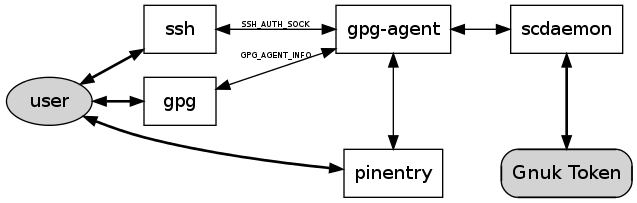
\includegraphics[width=.8\hsize]{image2013-gum/gnupg-friends.png}
\caption{GnuPGとGnuk Token}
\label{fig:gnupg-friends}
\end{figure}

\iffalse
GnuPGには簡易版1.4.xシリーズと、フル機能の2.0.xシリーズがありますが、
デスクトップ環境で使う場合は2.0.xシリーズの利用を推奨します。
\fi
% ソフトウェアとしてのGnuPG全体には、コマンドgpg / gpg2の他に、
% gpgv, gpgsmなどのツール、gpg-agent, scdaemonなどのデーモンが含まれます。

\iffalse
gpgとgpg-agentの関係は、コマンドgpgがユーザが起動するフロントエンドで、
gpg-agentが秘密鍵を扱うバックエンドとなっています。
gpg-agentはログイン時に自動的に起動されます。

scdaemonがGnuk Tokenと通信するプログラムです(SmartCardDaemon の略)。
scdaemonはgpg-agentから起動されます。

pinentryはパスワードを入力するためのツールで、gpg-agentから起動されます。

Gnuk TokenはGnuPGの内蔵のドライバで動きます。PC/SCを使う必要はありません。
PC/SCを使うこともできますが、ファームウェア・アップグレードの動作に悪影響があるので、
PC/SCは使わないことを推奨します。
\fi

\subsubsection{SSHについて}
あまり知られていませんが、
GnuPGのgpg-agentではssh-agentのサービスを同時に動作させることができます。
これにより、GnuPGの鍵を使ってSSHの認証を行うことができます。
Gnuk Tokenを使えば、GnuPGの電子署名や暗号のための秘密鍵だけでなく、ネットワークアクセスの
ための秘密鍵も統合して、独立のデバイスに分離して管理することができます。

\iffalse
\subsubsection{Gnuk Tokenに関するudevの設定}
たとえば、\verb|/etc/udev/rules.d/60-gnuk.rules|に図\ref{fig:gnuk-udev}の内容でrulesを記述します。\footnote{いちいちユーザが記述しなくても良いようにすべきです。bug 543217, 691392}

\begin{figure}[h]
\centering
\begin{Verbatim}[frame=single]
    SUBSYSTEMS=="usb", ATTRS{idVendor}=="234b", ATTRS{idProduct}=="0000",   \
    ENV{ID_SMARTCARD_READER}="1", ENV{ID_SMARTCARD_READER_DRIVER}="gnupg"
\end{Verbatim}
\caption{udevの設定}\label{fig:gnuk-udev}
\end{figure}

\subsubsection{gpg-agentの設定}
% \verb|.gnupg/gpg.conf|に use-agent| を追加します。

gpg-agentがssh-agentとして働くように、 \verb|~/.gnupg/gpg-agent.conf|
で\verb|enable-ssh-support| を設定します。

\subsubsection{デスクトップ環境の設定}
デスクトップ環境の設定として、gpg-agentが起動され、
本来のssh-agentが起動されないようにする必要があります。
このためにシステムとしてXsessionの設定をします。

Xsessionからssh-agentが起動されないようにします。
Debianの場合、
\verb|/etc/X11/Xsession.options|
で\verb|use-ssh-agent|の行をコメントアウトします。

Debian squeezeでは、seahorse-agentとgpg-agentが衝突します。
システム全体で、 もうseahorseは使わないという判断をする場合でも、
デスクトップ環境の各ソフトウェアとの依存関係が適切になっていないため、
seahorseパッケージだけを取り除くことができません。下記の対処をすることがよいでしょう。

\begin{commandline}
  # mv /etc/X11/Xsession.d/60seahorse /etc/X11/Xsession.d/x60seahorse
\end{commandline}

つまり、システム全体としてseahorse-agentを無効とします。

GNOME2の場合、gnome-keyringがssh-agentとして働くことを止める必要があります。
下記のコマンドで変更できます。

\begin{commandline}
  $ gconftool-2 --type bool --set /apps/gnome-keyring/daemon-components/ssh false
\end{commandline}


GNOME3ではgnome-keyringがさらにデスクトップに統合され、
独自の実装によりgpg-agentとssh-agentのサービスを行います。
しかし、この独自の実装はコンパチブルではなく、
GnuPGの有用な機能はサポートされず、Gnuk Tokenの利用ができません。
したがって、gnome-keyringの独自の実装によるgpg-agentとssh-agentのサービスを止め、
GnuPGのgpg-agentを利用する必要があります。これには、
下記のコマンドを起動します。

\begin{commandline}
  $ gnome-session-properties
\end{commandline}

そして"Startup Programs"のタブで、
``GPG Password Agent'' と ``SSH Key Agent'' のラジオボタンを外します。
\fi

\subsubsection{Gnuk Tokenの個人設定}
最初に、\verb|gpg --card-edit|でパーソナライゼーションを行います。
Gnuk Tokenにログイン名や公開鍵の置き場所のURLを登録できます。
そして、RSA 2048-bit鍵を3つ(それぞれ署名、暗号、認証用)用意し、
この鍵を書き込みます。
具体的な手順の詳細は、GnuPGのSmart Card HowTO\cite{gpg-sc-howto}や
"FST-01でGnukを使う"\cite{fst01handbook}
を参照してください。


\subsubsection{具体的な利用例: 署名}
ファイルに対する電子署名は、通常、
下記のように\verb|--clearsign|オプションで起動します。
最初の起動の場合、pinentryのウィンドウがポップアップし、
パスフレーズを聞いてきますので入力します。

\begin{commandline}
  $ gpg --clearsign <FILE>.txt
\end{commandline}

%
%約1.5秒後、ファイルに電子署名がなされ、\verb|<FILE>.txt.asc|ができます。

公開鍵への署名は、\verb|--sign-key|オプションで起動し、
サブセッションでパラメータを設定して行います。

\begin{commandline}
  $ gpg --sign-key <NAME>
\end{commandline}


Debianパッケージへの署名は、
.changesファイルと.dscファイルの二つのファイルに行われます。
%
特に指定しなければ、パッケージビルドの際、自動的にGnuPGが起動されて
署名が行われます。
\verb|-uc|オプションと\verb|us| オプションを指定して自動で署名を行わないようにもできます。
%
署名なしでビルドしたパッケージに、後で署名だけ行うには、
\verb|debsign|コマンドを用います。
%
必要であれば\verb|-k|オプションで鍵のIDを指定します。

Gitリポジトリへのコミットに対して署名するには、
\verb|git commit| の際、\verb|-s|オプションを使います。


\subsubsection{具体的な利用例: 認証(SSH)}
OpenSSHで利用するには、GnuPGの認証鍵から、
OpenSSHの形式の公開鍵を得る必要があります。
下記のコマンドで、SSHの公開鍵のフォーマットでデータが取得できます。

\begin{commandline}
  $ gpgkey2ssh <YOUR-KEY-ID>
\end{commandline}

ここで key IDとして16進数を指定する場合、全部大文字とする必要があります。
このSSHの公開鍵のデータをリモートのホストに登録します。
最初の認証に別の認証が使える場合には、直接、
\verb|ssh-copy-id|コマンドを使って登録できます。
%
また、
Debian開発者がDebianにSSH鍵を登録する場合は下記のようになるでしょう。

\begin{commandline}
  $ gpgkey2ssh <YOUR-KEY-ID> | gpg --clearsign | mail changes@db.debian.org
\end{commandline}


この設定ができたら、後は、SSH でリモートホストにアクセスできます。
認証には約1.5秒かかります。

\iffalse
\subsection{今後の開発}
Gnuk Tokenに関連した研究開発には、下記のものがあるでしょう。

\begin{itemize}
\item 利用に応じた環境の整備
  \begin{itemize}
  \item SSHのログイン先との通信での電子署名
  \item X.509クライアント証明書認証の安定化
  \item WindowsでのSSHとの相互運用
  \end{itemize}
\item 楕円曲線暗号(ECDSA / ECDH)のサポート
\item ChibiOS/RTに替えてChopstxの利用
\item 認証方式の研究開発
\end{itemize}

利用をより便利にする環境の整備が重要でしょう。
手元のGnuk TokenをSSHのログイン先で通信で利用する仕組み
(SSH のagent forwardingに相当する機能)があれば有用でしょう。
GnuPGはX.509にも対応しており、scute\cite{scute}
によりX.509クライアント証明書認証が利用できますが、
実験的側面が強いので、安定して利用できるようにする必要があるでしょう。
また、WindowsのSSH実装との相互運用の問題も解決する必要があります。

暗号方式の拡充として、楕円曲線暗号のサポートがあります。
OpenSSHでは既に楕円曲線暗号が利用できます。
GnuPGの開発版では楕円曲線暗号がサポートが組み込まれていて、
次のOpenPGPcard Protocolで楕円曲線暗号の利用について定義するよう議論されています。
開発版のGnukでは楕円曲線暗号の実装が進んでいます。

実装についての改善について、カーネルの置き換えを検討しています。
ChibiOS/RTは十分な機能を有する品質の高い自由ソフトウェアですが、
伝統的なRTOSのAPIを提供するものです。
伝統的なRTOSのAPIは実は因習なのではないかと疑問を持ち、
そもそもカーネルだけなのに ``OS'' と言うのがおかしいと考え、
現在、RTスレッドライブラリをChopstx\cite{chopstx}と名付けて開発をしています。
NeuGのスタンドアロン実装をChopstxに移植することができたので、
GnukもゆくゆくはChopstxに移植する予定です。

この他、PIN入力に代わる、ホストを経由しない認証の方式の検討もあるでしょう。
\fi

\iffalse
\subsection{おまけ: Gnuk Token開発の年譜}
この節では、おまけとして、Gnuk Tokenの関連の年譜を示します。

\begin{figure}[h]
\centering
\framebox{\begin{minipage}{.8\hsize}
\begin{description}
\item[2005年] OpenPGP card 1.0をドイツでもらう
\item[2008年] ATMega328でRSA 1024-bitの実装 (5秒くらい)
\item[2009年] ATMega328でOpenPGPcard Protocol 1.0の実験、発表
\item[2009年] OpenPGPcard Protocol 2.0が発表される
\item[2010年] Gnukの開発を開始
\item[2010年] GPF CryptoStickが開発され、製造販売が始まる
\item[2011年] GnuPGの開発に参加
\item[2011年] 真性乱数生成NeuGの開発を開始
\item[2011年] FST-01を開発
\item[2012年] Gnuk 1.0 をリリース
\item[2012年] FST-01の製造販売を開始
\item[2013年] RTスレッドライブラリ Chopstx の開発を開始
\end{description}
\end{minipage}
}
\caption{Gnuk Token開発の年譜}
\end{figure}

GnuPGの利用において秘密鍵の管理は重要な問題点として認識されており、
2005年には通信の仕様のOpenPGPcard Protocol 1.0が発表され、
これに準拠したICカードのOpenPGPcard 1.0が開発されました。
FSFEの会員カードはこれを用いています。
しかし、ICカードの利用にはICカードリーダが必要で、これは普及の問題があり、
カードは肌身離さずという運用が可能ですが、カードリーダの持ち運びは不便です。

そこで僕は2008年にUSBトークンを作れないか検討を始めました。
しかし、ICカード関連もそうですが、ハードウェアによる暗号関連の機能を搭載したデバイスは、
メーカと技術に関して非開示契約を締結しての技術開発が前提となることから、
自由ソフトウェアの開放型の開発には適さないことを身をもって経験しました。

特殊なハードウェアによる暗号関連の機能を用いず、
非開示契約を締結する必要のない一般のMCUを用いて、
USBセキュリティ・トークンを作る検討を進めました。
ATMega328の20MHzでRSA 1024-bitを約5秒で実行する実装を作りました。
OpenPGPcard Protocol 1.0の実装を一部行い実験し、2009年に発表しました。

2009年の同時期に、ホストPCとUSB接続するMCUを、
内部でOpenPGPcardのチップと接続する形態のUSBセキュリティ・トークンの開発が、
German Privacy Foundationにより開始されます。

OpenPGPcardは、通信の仕様は開示されていますが、
残念ながらICカード産業の慣習を反映し、そのファームウェアは自由ではなく、
それ自身の技術開発は制約がありました。

そこで、僕は、自由ソフトウェアによるUSBセキュリティ・トークンのファームウェアの実現、
と、OpenPGPcardよりも高い目標を掲げました。
単に利用できるだけではなく、研究開発に関して自由であることも重要だと考えました。

そして、2010年にSTM32F103をターゲットとすることを決定し、プロジェクトの名前をGnukとし、
セキュリティ・トークンのファームウェアを実現する自由ソフトウェアの開発を、
2010年9月に始めました。

その後、German Privacy Foundationはセキュリティ・トークンを製造し、
CryptoStickの名称で販売を始めました。

"動く"ということでは2010年10月にGnukの実装はあらまし動くようになりましたが、
実用として整備するために、Gnukの改良にだけでなく、いろいろな努力が必要となりました。

第一に、GnuPGにおけるOpenPGP cardのサポートは必ずしも十分ではありませんでした。
GnuPGの開発に参加して改善に取り組むことになりました。
2013年5月にリリースされたGnuPG 2.0.20ではだいぶ改善できています。

第二に、重要なのはRSAの計算(の高速化)だけではありませんでした。
暗号目的の使用に耐えうる品質の高い乱数生成が必要となりました。
このために、2011年に、
ADCの量子化誤差を主なエントロピー源とする真性乱数生成の実装、
NeuGの開発を行うことになりました。

第三に、ハードウェアについて、
既存のボードは大きくトークンとしての実用には疑問があるなどの声が寄せられたことから、
自由ソフトウェアの環境でPCB設計を行い、
2011年にFST-01と名付けて自由なハードウェア設計としてリリースしました。
しかし、さらに、ハードウェアは単に購入したい、との声が寄せられたことから、
2012年に製造販売を開始することとなりました。

冒険は続きます。
\fi

\begin{thebibliography}{1}
\bibitem{openpgp}
  {\footnotesize{
      J. Callas, et al., RFC4880, OpenPGP Message Format, 2007.
      }}
\bibitem{archlinux}
  {\footnotesize{
      Arch Linux Master Keys, \url{https://www.archlinux.org/master-keys/}
    }}
\bibitem{gpg-sc-howto}
  {\footnotesize{
      Rebecca Ehlers, et al., The GnuPG Smartcard HOWTO, 2005.
    }}
\bibitem{fst01handbook}
  {\footnotesize{
      FST-01でGnukを使う, \url{http://no-passwd.net/fst-01-gnuk-handbook/}
      }}
  \bibitem{chopstx}
    {\footnotesize{
        Threads and only Threads, \url{http://gitorious.org/chopstx}
      }}
  % \bibitem{scute} Scute, PKCS \#11 implementation for the GnuPG Agent, \verb|http://www.scute.org/|
\end{thebibliography}

\pagebreak
%-------------------------------------------------------------------------
\dancersection{Azure de Debian}{Kazumi HIROSE}

\subsection{はじめに}

Windows Azureは2009年からマイクロソフトが提供しているパブリッククラウドです。昨年6月にそれまで提供していた、Linuxが動作する仮想マシン(IaaS)が提供される事になりました。

本セッションでは、マイクロソフトの最近のOSSへの取り組みや、オープンソースに関連したWindows Azureの機能と、実際にDebianで活用する方法をご紹介します。

\subsection{Microsoftのオープンソースに対する取り組み}

この数年、Microsoftはオープンソースへの支持・支援を積極的に行なっています。

Linuxカーネルへのコミットメント、Apache Foundation VPであるGianugo Rabellino氏が入社、オープンソースコミュニティと協力する事を目的とした、MS Open Technologies社を設立しています。

HTML5やHTTP2.0を含む、150以上の標準化機関と400を越えるワーキンググループと共同作業を行っており、コミュニティにも積極的な支援をしています。

最近追加されたサービス・アプリケーションやSDKでは、自社プラットフォーム以外へも、iOSやAndroidのSDKを提供しています。

日本でも、WordPress/EC-CUBE/MODX/XOOPS Cube/Baser CMSなどのコミュニティや、PHP Matsuri/PHP Conference/Ruby Kaigi/Python Conference/Open Source Conferenceなどのイベントに協賛、支援をしています。

\subsection{Windows Azureについて}

ここではOSSやLinuxに関連する機能に絞り、最近のトピックスをご紹介します。


\subsubsection{管理ポータルの刷新}

Silverlightベースだった管理ポータルがHTML5ベースに作り変えられ、Linuxやスマートフォンからもアクセスできるようになり、日本語を含めた11ヶ国語で表示できるようになりました。

\subsubsection{新規リージョン提供の発表}

日本・オーストラリアにリージョンが展開されることが発表されました。

\subsubsection{"仮想マシン"の提供とLinuxのサポート}

Hyper-VのゲストOSを提供します。仮想マシンの対象OSにCentOS/Ubuntu Linux/suse Liunxが提供され、各ディストリビューションのサポートは、OpenLogic/Canonical/SUSEが対応します。

公式以外のイメージは、前述のMS Open TechnologiesによりVMDEPOTで提供されています。

\subsubsection{"Webサイト"の提供}

Sharedホスティング型PaaSの"Webサイト"が提供されました。ASP.NET/PHP/Node.js/Pythonで開発されたWEBアプリケーションを、FTP/Git/Mercurialやgithub/BitBucket/Codeplex/Team Foundation Service/Dropboxといったサービスからもデプロイできます。

また、ギャラリーにはWordPressなどがコミュニティにより提供されており、容易にサイト構築ができます。

\subsubsection{Windows Azure Xplat CLI Tool}

Node.jsベースでWindows AzureをCLI操作できるツールが提供されました。
Windows Azure CLI tool for Windows, Mac and Linux (Apache License)
\url{https://github.com/WindowsAzure/azure-sdk-tools-xplat}

\subsubsection{Windows Azure SDKの公開}

Java/Node.js/.NET/PHP/Python/RubyのSDKがApache Licenseでgithubに公開されました。
\subsection{AzureにおけるDebianのサポート状況}

Debianに限った話ではありませんが、AzureでLinuxを動作させるには、以下の要件を満たしている事が前提になっています。
\begin{itemize}
\item VHD形式の仮想HDDイメージである事
\item カーネルモジュールにHyper-V用モジュールが必要
\item WALinuxAgentが必要
\end{itemize}


\subsubsection{VHD形式の仮想HDDイメージである事}

Windows 8 Pro / Windows Server 2012/2008R2ではHyper-Vをインストールする事が出来ますので、そこでVHD形式のHDDイメージが作成できます。VMWare VMDKやVirtualBox VDIで作成されたイメージの場合、現時点ではNHCを用いて仮想HDDイメージの変換で対応できます。

\subsubsection{カーネルモジュールにHyper-V用モジュールが必要}

Linux integrated serviceと呼ばれていたソフトウェアが導入されている事が必要ですが、Linux3.2にGPLとして取り込まれた事で、Wheezyには既に導入されています。導入されているかの確認は以下の方法で行えます。

\begin{commandline}
$ sudo lsmod | grep hv
hv_utils               12986  0
hv_netvsc              18304  0
hv_storvsc             17423  2
hv_vmbus               32029  4 hv_storvsc,hv_netvsc,hid_hyperv,hv_utils
scsi_mod              162269  5 libata,sr_mod,sg,hv_storvsc,sd_mod
\end{commandline} %$

\subsubsection{WALinuxAgentが必要}

Windows Azure Linux Agent は、仮想マシンのCPU利用率やメモリ利用率などのモニタリング機能や管理機能を提供するPythonスクリプトです。
WA Linux Agent (Apache License) \url{https://github.com/Windows-Azure/WALinuxAgent}

Debianでは、Jessieにパッケージがありますので、APTのPIN機能でパッケージを借ります。

\subsubsection{/etc/apt/sources.list}
\begin{commandline}
deb http://ftp.jp.debian.org/debian/ wheezy main
deb http://security.debian.org/ wheezy/updates main
deb http://ftp.jp.debian.org/debian/ wheezy-updates main
deb http://ftp.jp.debian.org/debian/ jessie main
\end{commandline}

\subsubsection{/etc/apt/preferences}
\begin{commandline}
Package: *
Pin: release a=stable
Pin-Priority: 700

Package: *
Pin: release a=testing
Pin-Priority: 80

Package: *
Pin: release a=unstable
Pin-Priority: 90
\end{commandline}

\subsubsection{waagentのインストール}
\begin{commandline}
# apt-get install waagent/jessie
Reading package lists... Done
Building dependency tree
Reading state information... Done
Selected version '1.3.2-1' (Debian:testing [amd64]) for 'waagent'
... 中略 ...
Do you want to continue [Y/n]?
\end{commandline}

\subsubsection{ディスクイメージの準備}

汎用化ディスクイメージを作成します。このコマンドで環境に依存するファイルや設定をクリーンアップします。

\begin{commandline}
# waagent -deprovision
WARNING! The waagent service will be stopped.
WARNING! All SSH host key pairs will be deleted.
WARNING! Nameserver configuration in /etc/resolv.conf will be deleted.
WARNING! Cached DHCP leases will be deleted.
WARNING! root password will be disabled. You will not be able to login as root.
Do you want to proceed (y/n)? y
# shutdown -h now
\end{commandline}

\subsubsection{Windows Azureへアップロード}

Windows Azure Xplat CLIをインストールして、ディスクイメージをアップロードします。
\subsubsection{Node.jsの導入}

\begin{commandline}
# apt-get install python g++ make
# wget -N http://nodejs.org/dist/node-latest.tar.gz
# tar xzvf node-latest.tar.gz && cd node-v*
# ./configure
# make && make install
\end{commandline}

\subsubsection{Windows Azure Xplat CLIの導入}

\begin{commandline}
# npm install azure-cli -- g
$ azure
info:             _    _____   _ ___ ___
info:            /_\  |_  / | | | _ \ __|
info:      _ ___/ _ \__/ /| |_| |   / _|___ _ _
info:    (___  /_/ \_\/___|\___/|_|_\___| _____)
info:       (_______ _ _)         _ ______ _)_ _
info:              (______________ _ )   (___ _ _)
info:
info:    Windows Azure: Microsoft's Cloud Platform
info:
info:    Tool version 0.6.16
\end{commandline} %$


\subsubsection{Windows Azureのアカウント設定のダウンロードおよびインポート}
\begin{commandline}
$ azure account download // ブラウザが起動しダウンロードします。
$ azure account import [Downloaded File]
\end{commandline}

\subsubsection{ディスクイメージのアップロード}
\begin{commandline}
$ azure vm image create "Debian7.0-Wheezy-Minimal" --location "East Asia" --os Linux WheezyOnWA.vhd
info:    Executing command vm image create
+ Retrieving storage accounts
info:    VHD size : 30 GB
info:    Uploading 31457280.5 KB
Requested: 79.6% Completed: 79.0% Running:  92 Time:36m15s Speed: 11431 KB/s
\end{commandline} %$

アップロードしたディスクイメージは、インスタンスとして起動する事もVMDEPOTに登録する事もできます。

作成のイメージはVMDEPOTに登録していますので、是非使っていただければ幸いです。
\url{http://vmdepot.msopentech.com/Vhd/Show?vhdId=2427&version=2457}

\pagebreak
%---------------------------------------------------------------------------
% 佐々木
\dancersection{Dennou Club Library を Debian 公式パッケージにするには?}{佐々木洋平}
\label{sec:uwabami}

\subsection{はじめに - はなしの「まくら」}

Dennou Club Library(以下、DCL)は地球流体電脳倶楽部(\url{http://www.gfd-dennou.org/})の関係者が
長年にわたり蓄積してきた\footnote{%
  今回歴史を遡った所、1987 年頃にプロトタイプが公開されていた模様です。%
  ただ, 本当のプロトタイプは PC-8801 で動いていたという話(噂?)もありますので、正直いつからあるのか定かではありません(笑)%
}、欠損値処理や地図投影などの機能が標準的にサポートされた描画ライブラリです。
%
DCL は FORTRAN77 で書かれており,
これをベースに \texttt{f2c} によって生成されたコードに手を入れた C 版,  これを用いる Ruby 拡張ライブラリも提供しています
\footnote{%
  数値計算は FORTRAN, fortran, C で行なっても, その後のデータ解析までこれらの言語でやるのは結構シンドイです。
  「計算量自体が少ない場合。例えば C で 1 秒以内に済む計算
  が、Ruby では 1 分かかるかもしれない。しかし、そのためのプログラム開発
  に C では 5 時間かかり、Rubyでは 30 分程度で済むならどうだろう。もしも
  そのプログラムを実行するのが高々数10回程度としたら、Ruby を使うことはお
  かしな選択ではない\cite{RubiMa6}。」と、筆者も思っています。
}。
%
日本に限らず世界各地の大気海洋科学の研究者に用いられており、ソースコード
は全て公開され「無責任無保証の元で改変と再配布は自由に行なえる状況」にあ
ります。

しかしながら、長年の蓄積と当時の牧歌的な状況などからか、コピーライトやラ
イセンスは(上記文章は含まれているものの)あまり明確ではなく、このままでは
「フリーソフトウェア」と名乗って良いものか定かではありません。
%
本稿では、筆者が「DCL を Debian の公式パッケージとしたい!」と思って
行なった/行なっているアレやコレについてまとめてみます。

\subsection{%
  「地球流体電脳倶楽部」とは?
}

「地球流体電脳倶楽部」は, 主に地球惑星科学, 天文学における「流体」を研究
する分野の研究者と学生からなる草の根(もしくはボランティア)集団です
\footnote{%
  たまに誤解されますが、
  特定の資金源や専任スタッフが存在するわけではありません。%
}.
全国各地の有志から構成されており, 普段はネットワーク上で活動していることが多
い(active member は 20 名程?)です.
%
詳細に関しては
「地球流体電脳倶楽部について(\url{http://www.gfd-dennou.org/html/about/})」
あたりをご覧下さい.

我々は好んで Debian を使用しています。
%
我々の「ポリシー」%
\footnote{ポリシー: \url{http://www.gfd-dennou.org/html/about/policy.html}}
において
\begin{quote}
  研究教育のための情報は無料でなければならない \\
  少なくとも税金で運営されている国立大学、国立研究所が提供する情報は無料
  であるべきである。また、その情報の出所が明らかでなければならない。
  さらに、その情報の再配布が可能であることが望ましい。
\end{quote}
と掲げている通り、Debian ファンが多い集団
でもあったりします。
「無料」と掲げている点が悩ましい所ではありますが...。
%
現在、北大・京大・九大にサーバを設置し Debian のミラーをやっていたりしま
す。関係者が他の大学/研究機関へ異動し(機関の許可があれば)他にも増えるかも
しれません(減るかもしれません)。

\subsection{%
  事の発端
}

筆者は、地球流体電脳倶楽部で開発・配布しているソフトウェアを野良Debianパッ
ケージとして公開しています:

\begin{commandline}
  # sid, GPG: 0xAEE995F4
  deb http://www.gfd-dennou.org/library/cc-env/Linux/debian-dennou squeeze/
  deb-src http://www.gfd-dennou.org/library/cc-env/Linux/debian-dennou squeeze/

  # wheezy, GPG: 0xAEE995F4
  deb http://www.gfd-dennou.org/library/cc-env/Linux/debian-dennou squeeze/
  deb-src http://www.gfd-dennou.org/library/cc-env/Linux/debian-dennou squeeze/
\end{commandline}
%
自分が計算機にソフトウェアをインストールする際に
毎回ビルドするのが手間で作成/整理し始めたのですが、
最近は自分でリポジトリを用意するのが面倒になってきましたし,
「ライセンスに問題が無いならいっそ Official に入れてしまおう」と思いついたのが
事の発端です\footnote{%
  「Ubuntu のリポジトリは無いの?」
  という問い合わせが増えたのも理由の一つではあります
  (一応 PPA は有志によって用意されています)。
  実態は上記 apt リポジトリの(とあるタイミングでの) clone ですが。
}

\subsubsection{%
  Ruby まわりは upload できたけれど
}
ライセンスがクリアなソフトウェア(特に Ruby まわりのソフトウェア)に関しては、
既に Official に upload してあります。
代表的なのは
\begin{itemize}
\item %
  \texttt{ruby-netcdf}: NetCDF を Ruby で扱うライブラリ
  \footnote{
    PTS: ruby-netcdf, \url{
      http://packages.qa.debian.org/r/ruby-netcdf.html}
  }
\item %
  \texttt{ruby-grib}: ECMWF GRIB を Ruby で扱うライブラリ
  \footnote{
    PTS: ruby-grib, \url{
      http://packages.qa.debian.org/r/ruby-grib.html}
  }
\item %
  \texttt{ruby-lapack}: LAPACK の 1 to 1 wrapper
  \footnote{
    PTS: ruby-lapack, \url{
      http://packages.qa.debian.org/r/ruby-lapack.html}
  }
\end{itemize}
でしょうか。これらは BSD 2-Clause or Ruby's なので、
Official にアップロードするのには特に困りませんでした。

\subsubsection{%
  で「GPL 準拠」なの? それ、良いの?%
}

データの入出力、解析を行なうためのツールはちゃくちゃくと整理・Official への upload が進んでいた訳ですが、
肝心の描画ライブラリがなかなか進みません。
%
そもそも当時はライセンスが明確にされておらず、そもそも \texttt{debian/copyright} を書くことができませんでした。
しかしながら、FAQ \cite{DCL-FAQ} には
\begin{quotation}
  \noindent
  \textbf{DCL はフリーですか?} \\
  はい、フリーソフトウェアです。著作権は GNU Public License に準拠してお
  ります。因みにパッケージ内の CREDITS には版権を以下のように定めており
  ます。
  \begin{quote}
    本資源の版権は地球流体電脳倶楽部に属する。資源の利用にあたっては地
    球流体電脳倶楽部の定める規定にしたがっていただきたい。原則として、教育
    的目的の場合には自由に使用・改変して良いものとしている。
  \end{quote}
\end{quotation}
とあるわけです\footnote{``GNU Public License'' は typo. ではありません. 念のため}。

\subsection{%
  歴史を紐解く
}

というわけで、本当に GNU \underline{General} Public License (以下, GPL) 準拠%
になっているのか確認した上で、
\texttt{debian/copyright} 書いてみましょうか、という事になります。
これが明確になってないと ITP/RFS しにくいですし。

コードの大部分は
地球流体電脳倶楽部関係者によって開発・整理されているため、
Copyright holder が誰であるか問い合わせる/明確にする作業は着々と進んでいました
\footnote{%
  実際には Copyright が明記されていないコードに関して
  原作者に問い合わせ\texttt{ (c) GFD-Dennou Club } に変更/明記するだけです。
}。
...進んでいたのですが。

\subsection{%
  問題点
}
以下, 現状把握されている問題点を解決済の物も含めて解説してみます。


\subsubsection{%
  Numerical Recipe 由来: 解決済み%
}

乱数生成に関するコードの一部に Numerical Recipes 由来の SUBROUTINE が使われていました。
良く知られている通り Numerical Recipes のライセンスはフリーではありません
\footnote{%
  (自称を含めた)数値計算屋さんにはあまりちゃんと広まっていませんが、
  Numerical Recipes は、内容に関する批判もさることながら、%
  「この本を読んでコードを書くとコードが公開できない」という点において、%
  決して科学・教育に使ってはいけない本だと、筆者は考えます。
  ちなみに内容に関しては、読んでいないので批判できません。
  コードの質は一時に比較して改善されているらしいですね。
}。

そもそも FORTRAN77 には乱数ルーチンが無い(!)ため、些細な事ですが自前で実
装する必要がありました。デフォルトでは C の \texttt{rand()} を FORTRAN77
から呼び出しているだけであり、これが使えない場合の代替手段として提供して
いた SUBROUTINE でしたので、結局該当 SUBROUTINE を破棄することにしました。


\subsubsection{%
  Hershey フォント: 解決(?)
}

DCL では軸ラベル, タイトル等の描画等に Hershey フォントを使用しています。

Hershey フォントはHershey, A.V. が 1967 年に作成したベクタフォントで
す\cite{Hershey}。原論文は参照していませんが、その後 USENET でフォントデー
タが配布されており、その際のライセンスは

\begin{commandline}
  USE RESTRICTION:
        This distribution of the Hershey Fonts may be used by anyone for
        any purpose, commercial or otherwise, providing that:
                1. The following acknowledgements must be distributed with
                        the font data:
                        - The Hershey Fonts were originally created by Dr.
                                A. V. Hershey while working at the U. S.
                                National Bureau of Standards.
                        - The format of the Font data in this distribution
                                was originally created by
                                        James Hurt
                                        Cognition, Inc.
                                        900 Technology Park Drive
                                        Billerica, MA 01821
                                        (mit-eddie!ci-dandelion!hurt)
                2. The font data in this distribution may be converted into
                   any other format ((*EXCEPT*)) the format distributed by
                   the U.S. NTIS (which organization holds the rights
                   to the distribution and use of the font data in that
                   particular format). Not that anybody would really
                   ,*want* to use their format... each point is described
                   in eight bytes as ``xxx yyy:'', where xxx and yyy are
                   the coordinate values as ASCII numbers.
\end{commandline}
となっています
\footnote{%
  その後幾つか glyph が追加されていきましたが、
  現在 ghostscript に含まれている改良(悪?)版は,
  glyph を追加した人によって
  ``These are ``freeware'', not to be sold.'' という文言が追加されたため
  Debian では \texttt{non-free/gsfonts-other} で提供されています。
}。
さて, これはどういう扱いになるのでしょうか?

次期バージョンの DCL は GTK/Cairo を使って描画するように下層の入れ替えを
進めていますので、もしかしたらこの疑問は不要になるのかもしれません。%
ただ、昔の図の再現性が無くなるのはちょっと痛いです。

\subsubsection{%
  海岸線データ: 解決(?)
}

DCL では地図投影を行なった際に、地図を描画することができます。この際の海
岸線データの出所について、あまり明瞭に記載がされていません。日本付近の高
精細海岸線データに関しては、とりあえず配布物から抜いて、別途確認中です。

\subsubsection{%
  colormap: 解決(?)
}

現在 DCL で使用できる colormap の一覧は
\url{http://www.gfd-dennou.org/library/dcl/dcl-5.4.8/src/env1/colormap/colormap_gallery.html}
にあります。
%
幾つかの colormap は他のソフトウェアの colormap を\textbf{参考にして} 作っています。
(例えば, GNU Octave\cite{Octave}, IDV\cite{IDV}, NCL\cite{NCL} など)。
%

コードをそのまま持ってきた訳ではない,
出力結果を元に色調を手で合わせて作成された colormap なのですが、
この場合にはライセンスはどうなる/どうすべきなのでしょうね.
%
とりあえず、現状は配布物に同梱されていますが、抜くことも容易に可能な状況
にしてあります。

\subsubsection{%
  欲望との戦い: 引用して欲しいよね?
}

科学研究では論文を書く/書いた論文が引用される、というプロセスが重視される
ことが多いです。研究・教育におけるソフトウェア開発は(ソフトウェアそのもの
を研究する場合を除くと)、あまり評価されていません。これについて「使ったら
なるべく引用して欲しいよね」となるのが人情かもしれません。

DFSG-FAQ\cite{DFSG FAQ}, 10.g (draft 版ですので, 項目はまた変わるかもしれ
ません) には ``You have a valid concern.'' から続く, 以下の文言があります:
\vspace{-.5em}
\begin{quotation}
  \noindent
  Computer scientists often receive inadequate credit for their
  scientific contributions. But putting such a clause in the license
  would render your software non-free. Instead we suggest a note, not
  part of the license itself, reminding users of the rules of scientific
  propriety. Eg:
  \begin{quotation}
    \noindent
    SCIENTISTS: please be aware that the fact that this program is
    released as Free Software does not excuse you from scientific
    propriety, which obligates you to give appropriate credit!
    ...(略
  \end{quotation}
\end{quotation}
\vspace{-.5em}
ちょっとキツメの書きかたなので, どういう文章にするかは考える必要があるか
もしれません.

\subsection{%
  まとまらない%
}

これらの問題が解決した段階で、ようやくライセンスを「GPL 準拠」にしよう、
という話になるわけですが、現状では BSD 2-Clause にしたい、という意見が(開
発者の)大半を占めており、問題が無いのであればそうしましょう、ということに
なっています。
%
これは「大学で使っていたソフトウェアはそのままどこに行っても使えて欲しい」
という気持からです.

一方で、DCL とは(あまり)関係がありませんが「数値モデルを共同で開発しましょ
う」という際に、ライセンスについて
\vspace{-.5em}
\begin{quotation}
  有能な技術者が理解のない上官の下で孤立しているようなとき、外部ソフトウェ
  アの差分をその開発コミュニティにフィードバックすること自体は、まあ承認
  を得ることが可能であるけれど、その差分のライセンスに注目がいったら最後、
  職務著作であるからライセンス設定について然るべきものによる正当な意思決
  定をしなければならないという、反論不能かつ事実上実行不能な指示=リスク
  回避が行われることがままあるわけですね。

  そのときおおもとのソフトウェアが(L)GPLであってくれれば、差分が少なくと
  も(L)GPLでなければならないという制約がかかるので、意思決定がバイパスさ
  れます。ガバナンスが崩壊している組織においては、意思決定が不可能である
  ことがボトルネックですから、これで仕事ができるようになるわけです。まあ、
  要するに外圧スキームですが。
\end{quotation}
\vspace{-.5em}
という話もあって、個人的には LGPL-2+ あたりにしておいた方が良いかもしれな
い、とか思っていたりします。
%
まとまってませんが、そんなこんなで。

\vspace{-1.5em}
\begin{thebibliography}{2}
  {\footnotesize{
  \bibitem{Dennou}
    地球流体電脳倶楽部、
    \url{http://www.gfd-dennou.org/}

  \bibitem{RubiMa6}
    堀之内 武(著)、立石 孝彰(編)
    「数値計算と可視化」、
    Ruby Library Report 第5回、
    Rubyist Magazine、 No.{6}、
    \url{http://magazine.rubyist.net/?0006-RLR}

  \bibitem{DCL-FAQ}
    地球流体電脳ライブラリ Q and A 集,
    \url{http://www.gfd-dennou.org/arch/dcl/dcl-QA/dcl-QandA.html}
  \bibitem{Hershey}
    Hershey, A. V.,  1967:
    ``Calligraphy for Computers, Dahlgren, VA'',
    U.S. Naval Weapons Laboratory,
    \textit{NWL Report}, \textbf{2101}. NTIS AD662398.
  \bibitem{Octave}
    GNU octave:
    \url{http://www.gnu.org/software/octave/}
  \bibitem{IDV}
    IDV: \url{http://www.unidata.ucar.edu/software/idv/}
  \bibitem{NCL}
    NCL: \url{http://www.ncl.ucar.edu/}
  \bibitem{DFSG FAQ}
    DFSG and Software License FAQ (Draft):
    \url{http://people.debian.org/~bap/dfsg-faq.html}
  }}
\end{thebibliography}


\pagebreak
%-------------------------------------------------------------------------
\dancersection{自作描画ツール Linkdraw の紹介}{村越 俊克}

\subsection{はじめに}

私は、サーバやネットワーク周りの運用をしているエンジニアです。日々、運用をしていると様々な``手間''に遭遇します。そして、その都度いろいろな"ツール"を利用したり自作しては、ちょっとだけ楽をしております。今回は、Linkdraw という自作ツールを紹介します。

\subsection{Linkdraw}
"繋がりを描く"という名前の通り Linkdraw とは、アイテムとアイテム間の繋がりを描画する為のツールです。描画されたアイテムは、ドラッグアンドドロップで動かしたりハイパーリンクを埋め込む事も可能な為、ドキュメントやwiki 等の運用情報とリンクすることもできます。

以下は、サンプルです。

\begin{figure}[h!]
\centering
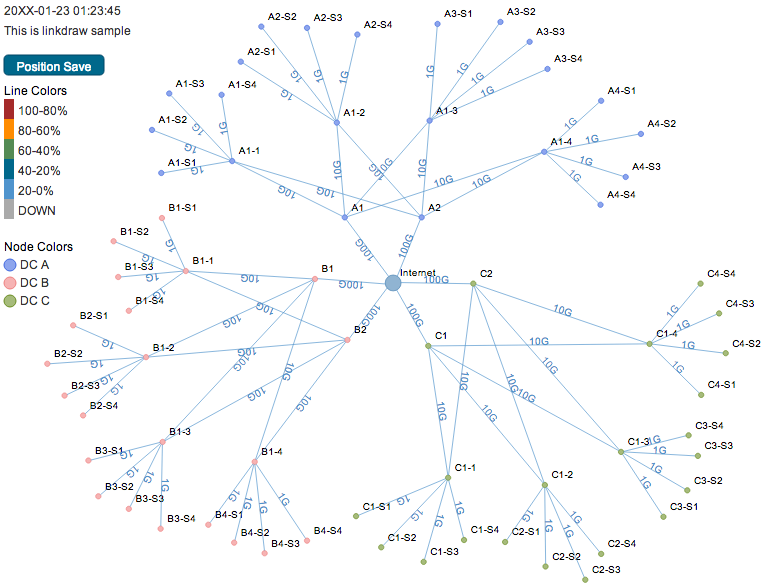
\includegraphics[width=0.8\hsize]{image2013-gum/mtoshilinkdraw2013061122150-img1.png}
\end{figure}
\pagebreak

\subsection{インストール}
Linkdraw は、現在、野良パッケージとなります。また、jQuery と d3 に依存しており jQuery は、公式パッケージですが d3 は、公式パッケージが存在しない為、こちらについても野良パッケージを作成しております。今回は、これらを使った説明となります。

まず、jquery をインストールします。

\begin{commandline}
$ sudo apt-get install libjs-jquery
\end{commandline} %$

次に、d3.js と linkdraw の野良パッケージをインストールします。

\begin{commandline}
$ wget http://linkdraw.org/deb/libjs-d3_3.1.10-1_all.deb
$ wget http://linkdraw.org/deb/libjs-linkdraw_0.2.4-1_all.deb
$ sudo dpkg -i libjs-d3_3.1.10-1_all.deb libjs-linkdraw_0.2.4-1_all.deb
\end{commandline} %$

コンテンツを設置したい場所(path/to/linkdraw)へ symlink を設置します。

\begin{commandline}
$ sudo ln -s /usr/share/javascript/jquery/jquery.min.js /path/to/linkdraw/js/jquery.min.js
$ sudo ln -s /usr/share/javascript/d3/d3.min.js /path/to/linkdraw/js/d3.min.js
$ sudo ln -s /usr/share/javascript/linkdraw/linkdraw.js /path/to/linkdraw/js/linkdraw.js
\end{commandline} %$

サンプルがインストールされているはずですのでこれらを setup.sh で設置します。

\begin{commandline}
$ cd /usr/share/linkdraw
$ bash utils/setup.sh /path/to/linkdraw
\end{commandline}

サンプルを確認してみましょう。

\begin{commandline}
  http://example.org/path/to/linkdraw/sample.html
\end{commandline}

\subsection{使い方}

まず、Linkdraw と依存関係にある jQuery と d3 を importします。
(外部から import できなければインストールで設置したローカルのsymlink で import)

\begin{commandline}
<script src=''http://code.jquery.com/jquery-1.10.1.min.js''></script>
<script>!window.jQuery && document.write('<script src=''/path/to/jquery.min.js''><\/script>')</script>

<script src=''http://d3js.org/d3.v3.min.js''></script>
<script>!window.d3 && document.write('<script src=''/path/to/d3.v3.min.js''><\/script>')</script>
<script src=''http://linkdraw.org/linkdraw.js''></script>
<script>!window.linkdraw && document.write('<script src=''path/to/linkdraw.js''><\/script>')</script>
\end{commandline}

次に、描画する HTML要素の id を指定して config ファイルのパス、ポジションファイルのパス、描画サイズなどを指定します。

\begin{commandline}
<script type=''text/javascript''>
$(function(){
     $(``#sample'').linkDraw({             //  描画するHTML要素の id を指定。
       ``configPath'': ``config.json'',      // 描画の為の設定ファイル。
       ``positionPath'': ``position.json'',  // ポジションを設定するファイル。
       ``positionWriter'': ``write.cgi'',    // ポジション情報を書き込む為の CGIプログラム .
       //''positionSave'': false,          // ポジション保存ボタンの表示。(デフォルト有効)
       //''zoom'': false,                  // 描画されたアイテムの拡大縮小。(デフォルト有効)
       //''drag'': false,                  // 描画されたアイテムの移動。(デフォルト有効)
       ``width'':  400,                    // svg 横(px)
       ``height'': 300,                    // svg 縦(px)
       ``interval'': 10                    // configPath で指定している設定ファイルの
                                         // 読込みインターバル(秒)。
     });
  });
</script>
\end{commandline}

以上が、HTMLの header 部分となります。

そして、 body の描画させたい箇所へ以下を追加します。

\begin{commandline}
<div id=''sample''></div>
\end{commandline}

以上で、HTMLの設定は、完了です。

次にconfigPath で指定した設定ファイル ``config.json'' を設置します。

\begin{commandline}
  vi config.json
\end{commandline}


サンプルとして以下を書いて保存します。(A と B という2つのノード間に線を1本引く設定)

\begin{commandline}
{
    ``lines'': [
        { ``source'': ``A'', ``target'': ``B'',''color'': ", ``width'': ``1'', ``descr'': ", ``link'': " }
    ]
}
\end{commandline}

次に、positionPath で指定したポジションファイル ``position.json'' を設置します。

このファイルは、空で構いません。 また、CGI プログラム によってポジションが保存される為、書き込み権限が必要となります。

\begin{commandline}
touch position.json
chmod 666 position.json
\end{commandline}

最後に、ポジションを保存する為のCGIプログラムを設置します。これは、linkdraw に付属している CGI (/usr/share/linkdraw/src/write.cgi)で構いません。(python2.6 以上で動作)

\begin{commandline}
chmod 755 write.cgi
\end{commandline}


以上で、必要なものが揃いました。

path/to/linkdraw 配下

\begin{commandline}
    jquery-1.10.1.min.js # jQuery(symlink)
    d3.v3.min.js         # d3(symlink)
    linkdraw.js          # linkdraw(symlink)
    sample.html          # HTML
    config.json          # 描画する為の設定
    position.json        # ポジションを保存するファイル
    write.cgi            # ポジションを保存する為のCGI
\end{commandline}

ブラウザで確認してみましょう。

\begin{commandline}
http://example.org/path/to/linkdraw/sample.html
\end{commandline}

以下の様に表示されたら成功です。

\begin{figure}[h!]
\centering
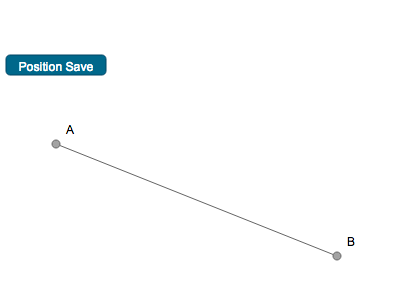
\includegraphics[width=0.4\hsize]{image2013-gum/mtoshilinkdraw2013061122150-img2.png}
\end{figure}

アイテムを動かして ``Position Save'' を押すとその時のポジションが保存されます。ブラウザで再読み込みを行うと次回からは保存された座標で描画されます。
また、 ``configPath'' で指定した設定ファイルの内容を更新していくことで描画するアイテムを制御することができます。設定ファイルの読み込みは、 ``interval'' で設定した値(秒) で行われる為、ブラウザの再読み込み(更新)は不要です。cron などで設定ファイルを定期的に置き換えることで自動更新が可能です。

\subsection{仕組み}

Linkdraw は json 形式で描画したいアイテムの情報を設定すると SVG で描画します。アイテムのポジションはランダムな座標が与えられブラウザ上に表示されます。表示されたアイテムはドラッグアンドドロップで動かすことが可能で、動かした後のポジションは保存することができます。保存されたポジション情報は、次回起動時に読み込まれる為、トポロジの形状を維持することができます。設定情報の json は、定期的に読み込まれ描画に反映されます。

\begin{figure}[h!]
\centering
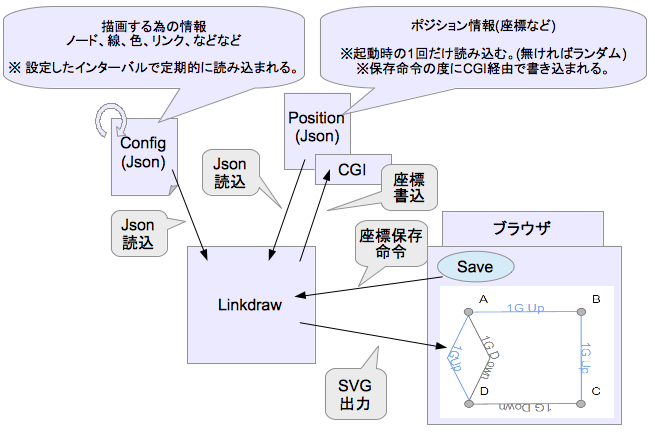
\includegraphics[width=0.6\hsize]{image2013-gum/mtoshilinkdraw2013061122150-img3.png}
\end{figure}


\subsection{まとめ}

Linkdraw を使うとアイテムとアイテム間の繋がりを簡単に描画することができます。現在私はLinkdraw を使ってデータセンタ内部の物理情報とその上に乗るトラフィックを自動描画しています。誰かが設置した機器や追加したケーブルが自動で反映されトラフィックも把握できるのでちょっとだけ楽をしています。Linkdraw についての情報は、日々更新していますので興味のある方は、\url{https://github.com/mtoshi/linkdraw/wiki} をご確認下さい。

\pagebreak
%-------------------------------------------------------------------------
% やまねさん
\dancersection{パッケージテストツール改善への取り組み}{やまねひでき}

\subsection{はじめに}

Debianにはパッケージの品質を向上するために各種ツールが開発されています。
パッケージビルドの依存関係を正常に保つため、クリーンルームビルドを行う"pbuilder/cowbuilder"、
Debianポリシーに沿った形でパッケージが作成されているかをチェックできる"lintian"、
パッケージのインストール・アンインストールをchroot環境で実施し問題を発見する"piuparts"などが代表的なものです。

この中で、あまり有効活用されていないのが"piuparts"です。その理由は"実施時間が膨大にかかる"
"デフォルトの出力が冗長であり、必要な情報を見つけ出すのが困難"という2点であると推測されます。
本稿では簡単なテストプログラムを作成し、piupartsにおける上記の問題を改善するアイデアを提案します。

\subsection{piuparts の実行時間と内容の分析}

現在、ITP中の"birdfont"という単体パッケージについて筆者の常用環境であるデスクトップPC上
(ストレージは一般的なHDDを利用)でpiupartsを実施し、時間を計測しました。piupartsのオプションは"-p"
(pbuilderで作ったbase.tgzを利用する)のみを選択しています。

\begin{commandline}
$ time sudo piuparts -p birdfont_0.18-1_amd64.deb
real 8m53.714s
user 0m18.525s
sys  0m5.576s

$ time sudo piuparts -p birdfont_0.18-1_amd64.deb
real 12m31.246s
user 0m18.661s
sys  0m5.444s
\end{commandline}
%$

ブレがあるが、おおよそ9-12分間の時間がかかるのがわかります(real)。
piupartsの動作としてはchroot環境にpbuilderのように最小限の"クリーンルーム"環境を作り、
必要なパッケージを逐一ダウンロードしてインストールを行います。
計測結果にあるように、一度のテストに最低でも10分近くを要する上、発生するパッケージの
インストール作業に伴うdisk I/Oが強烈で他の作業に支障が出るほどであることから、
開発者にとってはpiupartsの実施は相当のストレスであると予想できます。
一方、実際にプログラムが動作している時間は双方ともに18秒(user)と極小であることから、
何らかの形で"待ち時間"を減らしてやることで処理時間の改善が行えるであろうことが予想できます。

また、複数パッケージを生成するtwitterクライアント"hotot"についても同様にpiupartsを実施しました。

\begin{commandline}
$ time sudo piuparts -p hotot_0.9.8.13+git20130311-2_amd64.changes

real 37m24.258s
user 0m52.284s
sys  0m16.888s
\end{commandline}
%$

やはりrealと比較するとuser timeが極端に小さいことが見て取れます。

\subsection{SSD/tmpfsによる処理時間の削減}

ディスクアクセスが大量に発生していることから、HDDではなくSSD、または"tmpfs"
を利用した場合の速度を引き続きhototを対象に比較することにしました。

\begin{commandline}
$ time sudo piuparts -p -t /ssd hotot_0.9.8.13+git20130311-2_amd64.changes

real 2m3.441s
user 0m52.500s
sys  0m17.792s

$ time sudo piuparts -p -t /tmpfs hotot_0.9.8.13+git20130311-2_amd64.changes

real 1m41.406s
user 0m51.740s
sys  0m12.176s
\end{commandline}

双方とも大きな改善が認められます(37分 $\rightarrow$ 1.7〜2分)。
しかし、機器の増設と費用の関係上、Debianの開発者すべてがこの手法を手元のマシン上で採用できる訳でないため、
ソフトウェア側でも改善を引き続き試みました。

\subsection{COWアプローチの採用}

おおよそ、piupartsの動作は5つのステージに分けられます。

\begin{enumerate}
\item create base system with debootstrap (最小限の環境をdebootstrapで構築)
\item download related packages (関連パッケージのダウンロード)
\item extract \& install packages (パッケージの展開とインストール)
\item remove \& purge packages (パッケージの削除)
\item upgrade packages (パッケージのアップグレード)
\end{enumerate}

1については、一応既に考慮されており、pbuilderで作成したbase.tgzを利用するというオプションが用意されています。
ここで、筆者はpbuilderからの連想で、pbuilderよりも高速に動作が可能な"cowbuilder"に着目しました。
pbuilderに対するcowbuilderと同じアプローチでpiupartsもCOW(Copy On Write)を使ってディスクへの書き込みを減らす形で処理時間の短縮が図れると推測しました。

上川純一氏 (pbuilder及びcowbuilder 作者)によるJapan Linux Conference 2007 でのcowbuilderの論文(\url{http://lc.linux.or.jp/paper/lc2007/CP-06.pdf})を参
考にした所、いくつかのCOW実装(LVM2, user-mode-linux, qemu, fl-cow, unionfs, aufs)について比較を行っていました。
2007年当時、既存実装では一長一短だった部分があったためcowbuilderでは独自実装を行ったようですが、
筆者はこの中で取り上げられていたLinuxカーネルでのunionファイルシステム実装"aufs"が当時より好条件となっていることを発見しました。
メインラインには残念ながらマージされていないものの、安定して開発が継続されており、確認した所squeeze/wheezy/jessieのDebianのデフォルトカーネルで有効になっ
ているため利用は非常に簡易です。よって、本稿ではaufsを利用した改善を考察していきます。

\subsection{短縮可能な部分の洗い出しとテスト実装結果}

\begin{enumerate}
\item create base system with debootstrap (最小限の環境をdebootstrapで構築)
\item download related packages (関連パッケージのダウンロード)
\item extract \& install packages (パッケージの展開とインストール)
\item remove \& purge packages (パッケージの削除)
\item upgrade packages (パッケージのアップグレード)
\end{enumerate}

1 については、base.tgzの展開に時間がかかるので、最初にbase.cowを用意し、COWによってそれを下敷きにして利用することでこれを短縮します(数秒程度)。

2 については、ホスト側のパッケージキャッシュをunion mountすることでダウンロード時間を削減し、
かつダウンロードしたパッケージもunion mountすることで使いまわして毎回のダウンロードを行わないようにします。
birdfont を piuparts でテストした際にかかった時間は"Fetched 40.4 MB in 12s (3341 kB/s)"だったので12秒短縮
(世界平均が500kB/sぐらいなので、1分は短縮可能)となります。この点はテストするパッケージの依存関係が巨大で
あればあるほど短縮が可能です。

3 については特に変更する点は見出せませんでした。

4 については、uninstall と purge はそれぞれインストールして実施しているようですが、一旦 install ができた状態を COW で保持してその上に uninstall
用のレイヤーと purge 用のレイヤーを用意すればインストールは一回で済むので、ここを改善しました。
5については、現状ではパッケージバージョンの比較などを行っていないためダウングレードテストになってしまう場合がありますが、
作成ツール側ではアップグレード発生時以外はすべてキャンセルするなどして省略を図りました。

以上を元に、shell scriptでテスト実装"yasp"(Yet Another Simple/Speedy Piuparts)を作成し、テストを実施しました。

\begin{commandline}
$ time sudo yasp test hotot_0.9.8.13+git20130311-2_amd64.changes
kernel: Linux

for sid
caching .deb files for hotot-common...
caching .deb files for hotot-gtk...
caching .deb files for hotot-qt...
caching .deb files for hotot...
INSTALL: install package(s)...
debconf: delaying package configuration, since apt-utils is not installed
lsof: WARNING: can't stat() fuse.gvfs-fuse-daemon file system /home/henrich/.gvfs
      Output information may be incomplete.
Done
REMOVE: remove package(s)...
Done
PURGE: purge package(s)...
(snip)
Done
Package version 1:0.9.8.13+git20130311-4 (in sid)
Package vesrion 1:0.9.8.13+git20130311-2 (now you test)
1:0.9.8.13+git20130311-2 =< 1:0.9.8.13+git20130311-4
Skipping UPGRADE test...

PASS: install/remove/purge/upgrade test

real32m28.090s
user0m16.484s
sys0m11.872s
\end{commandline}
%$

上記のように、37分 $\rightarrow$ 32.5分と10\%以上の短縮が行えました。
メッセージ出力自体もdebconf絡みのエラーメッセージなど以外はシンプルになっているため、状況を把握しやすくなっています。
また、これをtmpfs上で実施した所、以下のように30秒弱でテスト自体を実施できました。

(作業ディレクトリをtmpfs上にした場合の結果)

\begin{commandline}
real 0m34.477s
user 0m16.820s
sys  0m7.772s
\end{commandline}

\subsection{結論}

インストールテストの大幅な作業時間の短縮にはSSDやtmpfsなどの高速なIOを提供できるデバイスを利用することが重要です。
しかし、ツール自体にも本稿で示唆したようにaufsを利用するなどして改善の余地があることがわかります。
可能な限りpiupartsへのフィードバックを実施し、よりDebianパッケージメンテナらが手軽にテストを実施できるよう改善を行いたいと思います。

\pagebreak
%---------------------------------------------------------------------------
% 西山さん
\dancersection{/etc/network/interfaces について}{西山和広}
\label{sec:etc-network-interfaces}

Debian でネットワークの設定を行うには /etc/network/interfaces ファイルに書く方法や NetworkManager を使う方法などがあります。
サーバー系では主に /etc/network/interfaces が使われていて、デスクトップ環境や無線 LAN のついたノート PC などでは NetworkManager が使われることが多いようです。

ここでは /etc/network/interfaces について説明します。

\subsection{/etc/network/interfaces とは?}

Linux ではディストリビューションごとにネットワーク設定の仕組みが異なっています。
Debian 系では /etc/network/interfaces がネットワークの設定ファイルです。
これは Red Hat Enterprise Linux や CentOS での /etc/sysconfig/network や /etc/sysconfig/network-scripts/ifcfg-eth0 などの設定ファイルに相当します。

/etc/network/interfaces は主に ifupdown パッケージで提供される ifup (ネットワークインターフェイス設定コマンド) と ifdown (設定解除コマンド) で使われます。
他にも NetworkManager や guessnet などのツールやスクリプトから参照されることもあるようです。
\footnote{resolvconf や wireless-tools や wpasupplicant などは後述する /etc/network/if-*.d/ の仕組みを使っているので、 /etc/network/interfaces ファイルを直接参照することはありません。}

\subsection{interfaces ファイルの構造}

interfaces ファイルは stanza (スタンザ) と呼ばれる固まりを並べる構造になっています。

例えば以下のような interfaces ファイルなら 6 個の stanza を含んでいます。

\begin{commandline}
# lo の auto stanza と iface stanza
auto lo
iface lo inet loopback

# eth0 の allow-hotplug stanza と iface stanza
allow-hotplug eth0
iface eth0 inet dhcp

# eth1 の allow-hotplug stanza と iface stanza
allow-hotplug eth1
iface eth1 inet static
    address 192.168.1.1
    netmask 255.255.255.0
\end{commandline}

最初の2個の stanza は lo という 127.0.0.1 や ::1 に対応するループバックインターフェイスの設定で、ここをいじることは普通はないと思います。

次の2個の stanza は eth0 という最初のネットワークインターフェイスは DHCP で自動で設定を取得しています。

最後の2個の stanza は eth1 というネットワークインターフェイスは 192.168.1.1 という IPv4 アドレスを設定しています。
address や netmask の行も iface stanza に含まれます。

\subsubsection{stanza とは}

stanza は "iface", "mapping", "auto", "source"\footnote{source stanza が使えるのは wheezy 以降のみです。} や "allow-"\footnote{allow-hotplug と allow-auto があるようです。}の行が stanza の始まりです。
stanza は 1 行だけのこともあれば複数行になっていることもあります。

以下の例ではそれぞれ 1 行ずつの stanza が 5 個あります。

\begin{commandline}
auto lo
iface lo inet loopback
allow-hotplug eth0
iface eth0 inet dhcp
allow-hotplug eth1
\end{commandline}

次の例では 3 行で 1 個の stanza になっています。
2 行目以降はインデントされていることもありますが、インデントはあってもなくてもかまいません。

\begin{commandline}
iface eth1 inet static
    address 192.168.1.1
    netmask 255.255.255.0
\end{commandline}

\subsubsection{コメント}

"\verb+#+"から始まる行はコメントです。
行の途中や行末に"\verb+#+"があっても設定値の一部になるだけでコメントにはなりません。

\subsection{stanza の種類}

\subsubsection{auto stanza}

auto stanza は \verb+ifup -a+ のコマンド実行時に up するインターフェイスの設定です。
複数設定したい場合は、1 行に複数並べてもいいし、複数回 auto stanza を書いても構いません。

\begin{commandline}
# 1行で書く例
auto eth0 eth1
\end{commandline}

\begin{commandline}
# 複数書く例
auto eth0
auto eth1
\end{commandline}

\subsubsection{allow-hotplug stanza}

allow-hotplug stanza は"\verb+ifup --allow=hotplug  eth0 eth1+"のように実行されたときに up する interface の設定です。\footnote{interfaces の man page では "allow-" stanza と説明されていて、 allow-auto は auto と同じ意味だと書かれています。}

udev で NIC などが認識されたタイミングで up するインターフェイスを設定します。auto だとデバイスの認識のタイミングの問題で up に失敗することがあるので、最近は allow-hotplug eth0 のようになっていることが多いようです。

etch や lenny では \verb+/etc/udev/rules.d/+ の中に、
squeeze や wheezy では \verb+/lib/udev/rules.d/+ の中に

\begin{commandline}
  SUBSYSTEM=="net", RUN+="net.agent"
\end{commandline}

という設定があり、\verb+/lib/udev/net.agent+ 経由で"\verb+ifup --allow=hotplug+"が実行されています。

\subsubsection{mapping stanza}
mapping stanza はプログラムの実行結果によって設定を切り替えたいときに使います。

\verb+/usr/share/doc/ifupdown/examples/+ 以下に、ノート PC で差した PC カードの MAC アドレスによって設定を変えたり (get-mac-address.sh)、特定の IP アドレスに ping が通るかどうかによって設定を変えたり (ping-places.sh) するサンプルファイルがあります。

\subsubsection{source stanza}

wheezy 以降の ifupdown パッケージでは source stanza というものが使えます。
interfaces ファイルの中で別のファイルを読み込む (include する) ものです。

例えば

\begin{commandline}
source /etc/network/interfaces.d/*
\end{commandline}

という設定を書けば /etc/network/interfaces.d/lo や /etc/network/interfaces.d/eth0 などに設定を分割して取り込むということも出来ます。

ただし NetworkManager などの別のツールやスクリプトで /etc/network/interfaces を直接見ている場合に問題が起きる可能性があるという議論\footnote{https://lists.debian.org/debian-devel/2013/01/msg00157.html}があるようです。

\subsubsection{iface stanza}

iface stanza は、IP アドレスなどのネットワーク設定を記述します。
"iface 名前 アドレスファミリ メソッド"という行で始まります。

iface stanza の最初の引数には eth0 などのような物理インターフェイス名を記述します。
物理インターフェイス名の代わりに、論理名で home と記述して"ifup ath0=home"のように使うこともできます。
\footnote{以前、/etc/network/run/ifstate (wheezy では /run/network/ifstate) に"lo=lo"とか"eth0=eth0"のようにあって、何の意味があるんだろうと思っていたのですが、"ifup ath0=home"とするとifstateに"ath0=home"と書き込まれていて、こういう場合に"="の左右が違うことがあるということを知りました。}

その他の設定については後述します。

\subsection{iface オプション}
アドレスファミリなどに関係なく共通で使えるオプションとして、以下の4種類があります。


\begin{description}
\item[pre-up] ネットワークを up する前に必要な無線 LAN 関係の設定などに使われる。
\item[up (post-up でも同じ)] ネットワークを up した後に追加で設定するのに使われたりインターフェイスの増減が影響するデーモンの再起動をしたり VPN の接続をしたり manual メソッドで up 処理を書くのに使われたりする。
\item[down (pre-down でも同じ)] VPN の切断をしたり切断対象のネットワークの DNS サーバーの設定を外したりする。
\item[post-down] 無線 LAN 関係の停止処理などに使われる。
\end{description}

実行の順序は、それぞれ以下のようになります。

\begin{description}
\item[ifup] pre-up → ifup の内部処理 → up (post-up)
\item[ifdown] down (pre-down) → ifdown の内部処理 → post-down
\end{description}

上記の設定と同じタイミングで \verb+/etc/network/if-*.d/+ に置かれたスクリプトも実行されます。
\footnote{run-parts で実行されるため /etc/cron*ly 以下などと同じくファイル名に"."などが含まれていると実行されません。}

スクリプトには iface stanza の情報として環境変数 IFACE, LOGICAL, ADDRFAM, METHOD, MODE, PHASE, VERBOSITY が渡されます。
他のオプションは"\verb+IF_+"で始まる環境変数で渡されます。

wireless-tools パッケージを入れたら"wireless-"で始まるオプションが使えたり、wpasupplicant パッケージを入れたら"wpa-"で始まるオプションを使えたり、resolvconf パッケージを入れたら"dns-"で始まるオプションが使えたり、ifenslave-2.6 パッケージを入れたら"slaves"オプションが使えたりするのは、この"\verb+IF_+"で始まる環境変数を"/etc/network/if-*.d/"以下のスクリプトで使っているからです。

以下ではパッケージで導入されるスクリプトと独自スクリプトの例について説明します。

\subsubsection{パッケージで導入されるスクリプトの例}
パッケージで導入されるスクリプトの例として、resolvconf パッケージを取り上げます。

resolvconf パッケージの説明には"resolvconf はシステムのネームサーバ情報を最新に保つためのフレームワークです。情報を提供するプログラム (ifup、ifdown、DHCP クライアント、PPP デーモン、ローカルのネームサーバなど) と、情報を使うプログラム (DNS キャッシュやリゾルバライブラリなど) との間に入ります。"と書いています。
ここでは ifup、ifdown に関係する部分だけ説明します。

resolvconf パッケージをインストールすると
\begin{enumerate}
\item /etc/network/if-up.d/000resolvconf
\item /etc/network/if-down.d/resolvconf
\end{enumerate}
というファイルが出来ます。

000resolvconf の内容をコメントや空行を除外して引用します。

\begin{commandline}
% egrep '^[^#]' /etc/network/if-up.d/000resolvconf | cat -n
     1  [ -x /sbin/resolvconf ] || exit 0
     2  case "$ADDRFAM" in
     3    inet|inet6) : ;;
     4    *) exit 0 ;;
     5  esac
     6  R=""
     7  if [ "$IF_DNS_DOMAIN" ] ; then
     8          R="${R}domain $IF_DNS_DOMAIN
     9  "
    10  fi
    11  if [ "$IF_DNS_SEARCH" ] ; then
    12          R="${R}search $IF_DNS_SEARCH
    13  "
    14  fi
    15  if [ "$IF_DNS_SORTLIST" ] ; then
    16          R="${R}sortlist $IF_DNS_SORTLIST
    17  "
    18  fi
    19  for NS in $IF_DNS_NAMESERVERS ; do
    20          R="${R}nameserver $NS
    21  "
    22  done
    23  echo -n "$R" | /sbin/resolvconf -a "${IFACE}.${ADDRFAM}"
\end{commandline}

まず1行目には /sbin/resolvconf の存在チェックがあります。
これはパッケージが削除されて設定ファイルだけ残っている時にエラーにならないようにするための処理です。

次に2から5行目では環境変数 ADDRFAM をチェックして IPv4 と IPv6 のときだけ続きの処理を実行します。
ADDRFAM や IFACE は iface の行の情報が設定されている環境変数です。

続きの設定はほぼ同じような処理の繰り返しなので、一番良く使われると思われる dns-nameservers について説明します。

/etc/network/interfaces ファイルの iface stanza で"dns-nameservers 192.168.0.1"や"dns-nameservers 192.168.0.1 192.168.0.2"のように設定します。

その設定が19行目で \verb+IF_DNS_NAMESERVERS+ という環境変数で参照されています。
他の設定も含めて resolvconf パッケージの独自設定には \verb+dns-+ を付けるようになっています。

設定を書く時に \verb+dns-+ を付け忘れて"nameservers 192.168.0.1"のように書いてしまうと resolvconf には反映されずに悩むことになるので注意が必要です。

このように環境変数で連携しているため、無効な設定があっても他で使っているかもしれないということで、設定ミスの自動チェックは難しいようです。

\subsubsection{環境変数の例}
独自スクリプトの例に入る前にスクリプトのなかで使える環境変数の例を紹介しておきます。

独自スクリプトを作成する時には、まず"up env $>$ /var/tmp/env.txt"などで使える環境変数を確認するのがおすすめです。
デバッグ中にも意図した通りの環境変数が設定されているかどうかを確認することをおすすめします。
"ifup -v eth0"のように"-v"付きで実行された場合は VERBOSITY が 1 になるので、その場合だけデバッグ用の出力を増やすようにするのもおすすめです。

まず、単純な"iface eth0 inet dhcp"だけの設定で"up env $>$ /var/tmp/env.txt"で保存した環境変数を例として載せておきます。
他にも pre-up や down や post-down でも 調べてみたところ、pre-up だと PHASE=pre-up になっているという違いがあり、down や post-down だと PHASE=pre-down や PHASE=post-down になっている他に MODE=stop になっているという違いがありました。

\begin{commandline}
METHOD=dhcp
MODE=start
LOGICAL=eth0
PHASE=post-up
ADDRFAM=inet
VERBOSITY=0
PATH=/usr/local/sbin:/usr/local/bin:/usr/sbin:/usr/bin:/sbin:/bin
IFACE=eth0
PWD=/
\end{commandline}


そして、もっと複雑な例としてブリッジ設定や後述する独自スクリプトの設定などが入っている時の例も載せておきます。

/etc/network/interfaces で

\begin{commandline}
iface br0 inet static
        # bridge
        bridge_ports eth0
        bridge_stp off
        bridge_fd 0
        bridge_maxwait 0
        # static
        address 192.168.253.29
        netmask 255.255.255.0
        gateway 192.168.253.1
        # iproute
        ip2-table 100
        ip2-net 192.168.253.0/24
        ip2-gateway 192.168.253.1
        post-up /etc/network/ip2-route.sh
        pre-down /etc/network/ip2-route.sh
        pre-up env > /var/tmp/env-$IFACE-$PHASE.txt
        post-down env > /var/tmp/env-$IFACE-$PHASE.txt
        # resolvconf
        dns-nameservers 192.168.253.1
\end{commandline}

のように設定している時に"/var/tmp/env-br0-pre-up.txt"は以下のようになります。
元の設定ファイルで"\verb+-+"で書いていても"\verb+_+"で書いていても環境変数では"\verb+_+"になるという点に注意が必要かもしれません。

\begin{commandline}
IF_BRIDGE_FD=0
METHOD=static
MODE=start
LOGICAL=br0
IF_IP2_GATEWAY=192.168.253.1
PHASE=pre-up
IF_BRIDGE_MAXWAIT=0
IF_ADDRESS=192.168.253.29
ADDRFAM=inet
VERBOSITY=0
PATH=/usr/local/sbin:/usr/local/bin:/usr/sbin:/usr/bin:/sbin:/bin
IF_IP2_NET=192.168.253.0/24
IF_GATEWAY=192.168.253.1
IF_METRIC=100
IF_NETMASK=255.255.255.0
IFACE=br0
IF_BRIDGE_STP=off
PWD=/
IF_IP2_TABLE=100
IF_BRIDGE_PORTS=eth0
IF_BROADCAST=+
IF_DNS_NAMESERVERS=192.168.253.1
\end{commandline}

\verb+IF_BRIDGE_+ で始まる環境変数は bridge-utils パッケージに含まれる
/etc/network/if-post-down.d/bridge
と
/etc/network/if-pre-up.d/bridge
使われます。

\verb+IF_IP2_+ で始まる環境変数は次で説明する独自スクリプトで使っています。

\subsubsection{独自スクリプトの例}

例として以前作成したインターネットへの経路が複数ある環境での設定スクリプトを載せておきます。

example では 192.168.0.1 側でも 192.168.0.1 側でも自宅サーバーを公開していて、リクエストが来た側に応答を返すような設定になっています。

\begin{commandline}
 % cat /etc/network/ip2-route.sh
 #!/bin/sh
 #
 # example:
 #
 #auto eth0
 #iface eth0 inet static
 #       address 192.168.0.2
 #       netmask 255.255.255.0
 #       gateway 192.168.0.1
 #       ip2-table 100
 #       ip2-net 192.168.0.0/24
 #       ip2-gateway 192.168.0.1
 #       post-up /etc/network/ip2-route.sh
 #       pre-down /etc/network/ip2-route.sh
 #auto eth1
 #iface eth1 inet static
 #       address 192.168.1.2
 #       netmask 255.255.255.0
 #       ip2-table 101
 #       ip2-net 192.168.1.0/24
 #       ip2-gateway 192.168.1.1
 #       post-up /etc/network/ip2-route.sh
 #       pre-down /etc/network/ip2-route.sh
 #

 [ -n "$IF_IP2_NET" ] || exit 0
 [ -n "$IF_IP2_TABLE" ] || exit 0
 [ -n "$IF_IP2_GATEWAY" ] || exit 0

 if [ "$VERBOSITY" -eq 1 ]; then
         set -x
 fi
 case "$PHASE" in
         *up)
                 ip route add $IF_IP2_NET dev $IFACE src $IF_ADDRESS table $IF_IP2_TABLE
                 ip route add default via $IF_IP2_GATEWAY table $IF_IP2_TABLE
                 ip rule add from $IF_ADDRESS table $IF_IP2_TABLE
         ;;
         *down)
                 ip rule del from $IF_ADDRESS table $IF_IP2_TABLE
                 ip route del default via $IF_IP2_GATEWAY table $IF_IP2_TABLE
                 ip route del $IF_IP2_NET dev $IFACE src $IF_ADDRESS table $IF_IP2_TABLE
         ;;
 esac

 exit 0
\end{commandline} %$

まず ip2-net, ip2-table, ip2-gateway のすべてを必須設定として、抜けがある場合は何もしないようにしています。

次に VERBOSITY をチェックしています。
ここでは ifup -v eth0 のように実行された時に後続のコマンドが実際にどういうコマンドラインで実行されるのかを表示するようにして、デバッグしやすくしています。

最後に up か down かに応じて ip コマンドを実行しています。

この設定ファイルを /etc/network/if-up.d/ と /etc/network/if-down.d/ の中にシンボリックリンクを作成しても良かったのですが、この例では /etc/network/ip2-route.sh に置いて、post-up と pre-down で実行するようにしています。
スクリプトをどう設置するのかは管理しやすい方法を選べば良いと思います。

スクリプトの説明はここまでです。
次からは /etc/network/interfaces の設定の説明に戻ります。

\subsection{inet アドレスファミリ}
IPv4 のネットワーク設定です。

\subsubsection{loopback メソッド}

\begin{commandline}
iface lo inet loopback
\end{commandline}

のことです。

iptables の設定に iptables-restore を使っているのなら、

\begin{commandline}
 # The loopback network interface
 auto lo
 iface lo inet loopback
   pre-up /sbin/iptables-restore < /etc/network/iptables.txt
\end{commandline}

のように lo の pre-up に設定しておけば他の interface が up される前に設定できていいかもしません。

\subsubsection{static メソッド}

address と netmask は必須です。

broadcast と network は address と netmask から自動設定可能なので、わざわざ書いて間違える可能性を増やすよりも省略しておく方がおすすめだと思います。

gateway も設定することが多いです。

\subsubsection{manual メソッド}

up や down などで全部自前で設定するときや "/etc/network/if-*.d/" 以下のスクリプトで設定する時などに使います。

bonding の slave 用 NIC に NetworkManager などが余計なことをしないように"iface eth1 inet manual"だけ書いておくという使い方も可能です。

\subsubsection{dhcp メソッド}

dhclient などで dhcp クライアントとしてネットワークを設定します。

\subsection{inet6 アドレスファミリ}
IPv6 のネットワーク設定です。

端末として接続するだけなら自動設定されることが多いので、わざわざ書くことは少ないかもしれません。
ルーターやサーバーなどで固定 IP アドレスを付けたり、トンネルで接続する場合に書くことになります。
接続方法によって設定内容が変わってくるので、詳細は省略します。

\subsection{設定書き換え時の注意}

ネットワーク接続中に /etc/network/interfaces を書き換えるのはあまりお勧めしません。

ifdown のときにも /etc/network/interfaces を見て何をするかが決まっているので、dhcp を static に書き換えてから /etc/init.d/networking restart をしてしまうと、dhcp クライアントのプロセスが残ってしまって、いつの間にかIPアドレスが変わって悩む、という現象が起きることがあるので注意が必要です。
たとえば他にも up で route add されていることを前提にして down に route del を書いていると、手動で up に書いた処理を実行しないと down の処理でエラーになるというような問題があります。

安全な方法としては ifdown で停止した後で /etc/network/interfaces を書き換えて、 ifup するという手順になります。

\subsection{参考文献}
\begin{enumerate}
\item %
  {\footnotesize{
      man interfaces で参照出来る interfaces(5) の man page
    }}
\item %
  {\footnotesize{
      Debian リファレンスの 第5章 ネットワークの設定 \url{http://www.debian.org/doc/manuals/debian-reference/ch05.ja.html}
    }}
\end{enumerate}

\pagebreak
%---------------------------------------------------------------------------
% 伊藤さん
\dancersection{ngraph-gtk で楽々グラフ作成}{伊東宏之}
\label{sec:ngraph}

5 月にリリースされた Debian 7.0 ``Wheezy'' から ngraph-gtk が公式パッケー
ジとして提供されるようになりました。Ngraph は MS-DOS の時代から利用されて
きた歴史あるグラフ作成プログラムです。現在は Windows 用がフリーウェア、
unix 用が GPL version 2 のフリーソフトとして配布されています。ngraph-gtk
はこの unix 用のソースを元に GTK+ 用に移植したものです。当初はウィジェッ
ト・ツールキットを Motif から GTK+ に変えただけでしたが、その後個人的に使
いやすいように機能追加、仕様変更を行なったため、今では外観や機能にだいぶ
違いが出てきました。

\subsection{概要}
ngraph-gtk は x-y グラフを作成するプログラムです。簡単な操作で綺麗なグラ
フを作成することができます。また、数式変換機能や任意関数でのフィッティン
グもできますので、簡単なデータ解析にも使えます。もちろんグラフのキャプショ
ンを作成する機能もありますし、作成したグラフは PostScript, PDF, SVG, PNG
などにエクスポートできますので、 Inkscape など他のソフトでさらに編集した
り、TeX の文章に貼り付けたりすることもできます。さらに sh 互換のスクリプ
ト言語を使用して機能を追加したり、グラフの自動作成も可能です。

ngraph-gtk を使ったグラフの作成は 1. データを用意する、2. ngraph-gtk でデー
タを開く、 3. 必要に応じて、データの変換やフィッティングの設定などを行う、
4. 軸のラベル、キャプションなどで体裁を整える、という手順になります。
ngraph-gtk-doc パッケージには詳しい日本語マニュアルが含まれており、その中
の"2. チュートリアル"を読めば基本的な使い方は習得できるはずです。基本的
な使い方はそちらを参照していただくことにして、ここではマニュアルに記述さ
れていない仕様やオリジナルとの相違点などを多く記述したいと思います。ぜひ
ngraph-gtk や ngraph-gtk-doc パッケージをインストールして、プログラムを動
かしたり、ドキュメントに目を通したりしてみてください。

\subsection{データファイル}

\subsubsection{一般的なデータ}
ngraph-gtk は ascii テキストで記述されたデータファイルをグラフに描画するとい
う思想で作られています。例えば $y=x^2$ のようなグラフを描かせる時でもデー
タファイルを用意する必要があります。データファイルは"データ"メニューの
"追加"で描画用のデータとして設定できます。標準の設定では半角スペース、
水平タブ、コンマ ``,''、カッコ``('', ``)'' のいずれかを区切り文字として、
第 1 カラムが $X$、第 2 カラムが $Y$ のデータとして読み込まれます。区切り
文字の設定はファイル設定ダイアログで設定を変えることができますが、指定で
きるのは表示可能な ascii 文字のみです。また区切り文字が連続する場合はまと
めて一つの区切りと解釈されます。例えば下記のような行は第1カラムが 2、第2
カラムが 4 となります (区切り文字設定がデフォルトの場合) 。

\begin{verbatim}
2, , , 4
\end{verbatim}

データ設定ダイアログで"CSV形式"にチェックすると上記の行は第1カラムが 2、
第2、第3カラムが 欠損、第4カラムが 4 となります。"CSV形式"という表記は
誤解を招きやすいのですが、半角スペース以外の区切り文字については連続して
いても一つの区切りとして扱わないという設定で、よくデータの交換に使われる
CSV形式とは必ずしも互換ではありません。例えば " (ダブルクォート) で囲まれ
た数値は正常に読み込めません。
% "

X が等間隔で Y のデータしかないデータファイルの場合 X のカラム指定を 0 に
するとテータを読み込んだ順に 1, 2, 3... が X の値になるので、このようなデー
タも問題なく描画できます。

文字列から浮動小数点への変換は strtod(3) を使用しています。これにより
strtod(3) がサポートする 10 進数、16 進数、無限 (INF, INFINITY)、NAN を読
み込むことができます。ただし ngraph-gtk では無限をサポートしていないので、
無限は NAN として扱われます。また strtod(3) で変換できなかった場合
``CONT'', ``BREAK'', ``UNDEF'', ``='', ``$|$'' のいずれかであればデータとし
て読み込まれます。``CONT'', ``BREAK'', ``='', ``$|$'' は欠損データとして扱
われますが、直線や曲線のプロットの場合 ``BREAK'', ``='' の前後で線が分割
されます。``UNDEF'' は未定義値として扱われます。これらの文字列の読み込み
時には大文字・小文字は区別されません。

\subsubsection{矩形、対角線、矢印プロット用データ}

ngraph-gtk では矩形や矢印のプロットも可能ですが、この場合データファイルの形式
が変わります。例えば下記のデータを X カラムを 1、Y カラムを 4 として、対
角線でプロットすると (0, 1) から (3, 4) に線が引かれます。すなわち Y カラ
ムとして指定されたデータは Y 座標ではなく、対角線の終点あるいは矩形の反対
側の角の X 座標となります。

\begin{verbatim}
0, 1, 2, 3, 4
\end{verbatim}

\subsubsection{誤差棒プロット用データ}

誤差棒のプロットも可能ですが、この場合もデータファイルの形式が変わります。
例えば下記のデータを X カラムを 1、Y カラムを 3 として、横誤差棒でプロッ
トすると (1, 3) から (-2, 3) に誤差棒が引かれます ($1 = 0 + 1, \ -2 = 0
+ (-2)$) 。一方、縦誤差棒でプロットすると (0, 7) から (0, -2) に誤差棒が
引かれます ($7 = 3 + 4, \ -2 = 3 + (-5)$) 。誤差棒の両端につく線の長さは
データ設定ダイアログの"サイズ"で変えることができます。

\begin{verbatim}
0, 1, -2, 3, 4, -5
\end{verbatim}


\subsubsection{日付データ}

ngraph-gtk では日付データもプロットすることができますが、ちょっとコツが必
要です。具体的には日付として扱いたい数値を MJD (修正ユリウス日
\footnote{1858年11月17日0000UT からの日数。}) に変換する必要があります。
このために数式変換の関数には $MJD({\rm year, month, day})$ および
$UNIX2MJD({\rm time})$ という関数が用意されています。例えば次のようなデー
タがあった場合、区切り文字に ``/'' を追加してX軸の数式変換を ``MJD(\%1,
\%2, \%3)'' とします。

\begin{verbatim}
2013/06/28 0
2013/06/29 1
2013/06/30 2
\end{verbatim}

次にX軸の"スケール-スケール法"を"MJD"にします。これで軸のナンバリング
に日付が表示されるようになりますが、表示が混み合って見難くなることがある
ので軸設定ダイアログで"目盛数字-位置-方向"を"軸と斜交1"などに設定して
おくのがお勧めです。日付の表記は"目盛数字-フォーマット-日時書式"で
strftime(3) とほぼ同様の書式を使って指定することもできます。

日付のデータが ``2013-06-29'' のような書式で与えられている場合は、区切り
文字に ``-'' を追加することで同様に描画できますが、この時他のカラムに負の
値を示す ``-'' があるとこれも区切り文字として解釈されてしまいます。今のと
ころこの現象を回避することはできないので、あらかじめ awk などを使って書式
を変換しておくことになります。

\subsection{数式変換機能}

読み込まれたデータは数式変換機能により指定した数式で変換してからプロット
することができます。数式はデータ設定ダイアログで指定できます。

数式変換機能は Ngraph のソースは使用せずに完全に新しく書き直しています。
従来は数式設定時にはスキャナが数値リテラルや定数、演算子などのトークンを
1 バイトの識別子や浮動小数点に変換するのみで、構文解析は計算時に毎回行わ
れるようになっていました。新しいコードでは数式設定時に構文木の生成まで行
い、グラフ描画前に簡単な最適化を行なってから実際の計算が実行されます。こ
れにより計算速度が大幅に向上し、また数式設定時に文法エラーのチェックも行
われるようになりました。また、代入可能な変数や配列が使用可能になったり、
各種関数が追加されたりという機能向上も行われています。

\subsubsection{演算子}

数式変換では四則演算や各種関数を使用できます。一部の演算子は一般的な表記
と異なるので、注意が必要です。例えば代入演算子は $:=$、剰余演算子は
$\backslash$ を使います。また階乗を計算する $!$ や、べき乗を計算する $^\wedge$
などの演算子も使うことができます。論理否定演算子は存在しないので $NOT()$
関数を使用します。

\subsubsection{変数と配列}

変数は $e$ 以外のアルファベット 1 文字が使えます ($e$ はネイピア数として
定数で使われているため) 。また変数 $x$, $y$ に値を代入することは可能です
が、データ読み込み時に指定したカラムのデータで上書きされます。変数は 0 で
初期化されているので、初期化のための代入は必ずしも必要ではありません。な
ぜ変数に使えるのがアルファベット1文字かというと、複数文字の変数を使える場
合、定数の綴りを間違えた時に変数と解釈されて間違いに気づきにくくなるとい
う点と、現状では数式変換には 1 行の数式しか記述できないため 1 文字の変数
でもわかりにくくなることはないだろうと考えたためです。

ngraph-gtk では配列も使うことができます。配列名は添字のための [\ ] で定数
と区別できるため、\% かアルファベットで始まり、\_ かアルファベット・数字
で構成される任意の長さの文字列を使うことができます。

\subsubsection{関数定義}

数式変換で独自の関数を定義することもできます。関数定義は下記の様な書式で
行います。

\[
 \mathrm{def\ \ func(a,\ @b)\ \{c:=a*b[0];\ sin(c)\};\ a[0]:=PI;\ func(1/2,\ a)}
\]

2番めの仮引数のように @ をつけると引数が配列であることを表します。関数の
戻り値は最後に評価された式の値になります。この例では$\sin(1/2\times\pi)$
を計算することになるので、式全体の値は $1$ になります。変数はすべてローカ
ルスコープで、グローバル変数はないので、関数に値を渡すときは引数か、メモ
リー関数を使うことになります。

\subsubsection{最適化}

数式変換では描画する前に簡単な最適化を行います。最適化では定数を数値に変
換、数値のみの項は事前に計算、数値による割り算は掛け算に変換といった処理
を行なっています。例えば式 \ref{Eqn:opt} は式 \ref{Eqn:opt2} のように最適
化されます。

\begin{eqnarray}
 1 + 2 + 3 + 4 + 5 + 6 + 7 + 8 + 9 + 10 + x / 10 \label{Eqn:opt}\\
 = 55 + x \times 0.1 \label{Eqn:opt2}
\end{eqnarray}

一方、式 \ref{Eqn:no_opt} のように書いた場合、式 \ref{Eqn:no_opt2} の様に
扱われるため足し算に関しては最適化は行われません。

\begin{eqnarray}
 x / 10 + 1 + 2 + 3 + 4 + 5 + 6 + 7 + 8 + 9 + 10  \label{Eqn:no_opt} \\
 = (((((((((((x \times 0.1) + 1) + 2) + 3) + 4) + 5) + 6) + 7) + 8) + 9) + 10)  \label{Eqn:no_opt2}
\end{eqnarray}

\subsubsection{浮動小数点の誤差}

ngraph-gtk ではすべての計算は倍精度浮動小数点で行われますが、よく知られて
いるように浮動小数点の計算では誤差に注意が必要です。例えば $0.5 - 0.4 =
0.1$ですが、ngraph script (詳細は後述) の iexpr コマンドで調べると $0.5
- 0.4$ は$0.1$ と等しくないことになってしまいます。

\begin{commandline}
 Ngraph$ iexpr '0.5-0.4::0.1'
 0
\end{commandline}
%$
\noindent
このような場合は $EQ()$ 関数で比較する桁数を指定すると期待通りの結果を得
られることが多くなります。

\begin{commandline}
Ngraph$ iexpr 'EQ(0.5-0.4, 0.1)'
0
Ngraph$ iexpr 'EQ(0.5-0.4, 0.1, 13)'
1
\end{commandline}

\noindent
2番めの実行例のように $EQ()$ 関数の第3引数で比較の桁数を13桁に指定すると、
14桁目が四捨五入されるため $0.5 - 0.4$ が $0.1$ と等しいという結果が得ら
れます。

\subsubsection{矩形、対角線、矢印、誤差棒プロットの数式変換}

これらのプロットでは、1行のデータに対して、誤差の上限・下限のように2回
数式変換が実行されます。この2回の呼び出しは定数 $FIRST$ で区別できます
(1回目の呼び出しは $FIRST$ が真) 。例えば次のようなデータを $3\pm0.2$ の
誤差棒でプロットするときは $IF(FIRST, \%02 + \%03, , \%02 - \%03)$ とい
う数式が使えます。数式変換で $y$ を使っていないのは、誤差棒プロットのデー
タフォーマットに従って、1回目の呼び出しでは $y=3+0.2$、2回目は $y=3+0$
となるので、数式変換使用時はわかりにくくなるためです。

\begin{verbatim}
1, 3, 0.2
\end{verbatim}

なお、この複数回呼び出される数式はすべて独立した数式として扱われています。
そのため、下記の式 (\ref{Eqn:FIRST}) のように変数を使って複数の呼び出しの
間で値を共有することはできません。このような場合は式 (\ref{Eqn:MEMORY})
のようにメモリー関数を使うことができます。メモリー関数はすべての数式変換
で共有されるので、複数のデータファイル間で値をやり取りすることもできます。

\begin{eqnarray}
 IF(FIRST, a := 1, a * 2) \label{Eqn:FIRST}\\
 IF(FIRST, M(0, 1), RM(0) * 2) \label{Eqn:MEMORY}
\end{eqnarray}

\subsubsection{その他}

式は ``;'' を区切りとして、複数記述することができます。最後の式の値が数式
変換の結果として使用されます。複数の式を記述する別の方法として
$PROG1()$, $PROG2()$, $PROGN()$ 関数を使用することもできます。例え
ば $DIF(y)$ とほぼ同様の計算は $PROG1(y-a, a:=y)$ の様に記述できます。
ngraph-gtk version 6.06.09 までは式の終端を表す記号として ``='' が使われ
ていたため代入や比較の演算子には記号 ``:'' を使用していました(:, ::,
$>$:, +: など) 。しかし、使っていてちょっとわかりにくい印象だったので
6.06.10 以降は代入演算子として ``:='' (Pascal と同じ) 、比較や自己代入演
算子は C と同じ表記が使えるようにしました。

ngraph-gtk の数式変換には制御構造の構文がありません。条件分岐や繰り返しは
$IF()$ や $FOR()$ などの関数を使用します。関数の引数では式の終端を表す
``;'' は使用できないので、複数の式を実行するためには $PROG1()$ 関数などを
使用します。なお $FOR()$ 関数では関数呼び出し時に繰り返しの回数が決まっ
てしまいます。これは数式変換の実行を中断する機能がないので、無限ループに
なった時プログラム自体を強制終了させる以外に停止手段がないためです。


\subsection{ngraph script}
\subsubsection{ngraph shell}

ngraph-gtk には ngraph shell というインタープリターがあり、このシェルで
ngraph script という言語を実行できます。マニュアルから引用すると"ngraph
スクリプトの文法は、UNIXの sh (シェル) からジョブ制御機能を取り去り、オ
ブジェクト操作命令を追加したもの"で、機能や実行速度の面から複雑な処理は
外部のプログラムに任せるという思想で作られています。"ジョブ制御機能を取
り去り"とあるとおり、コマンドをバックグラウンドで実行することはできませ
ん。またパイプも各プロセスはひとつずつ順に起動され、データは作業ファイル
経由で受け渡されます。

ngraph-gtk  ではグラフは  ngraph  オブジェクトの集合で構成されており  ngraph
script から各オブジェクトの設定を変更できますのでGUI を全く使わずにグラフ
を書くことも原理的には可能です。しかし、グラフを出力するためには多くの設
定や操作を行う必要があるため、すべて手動でグラフを作成するのはあまり現実
的ではありません。実際には他のプログラムからスクリプトを出力してグラフの
自動作成や作成支援を行ったり、グラフ設定の一部を手動で変更するというよう
な使い方が一般的と思います。

例えばすべてのデータで線の太さを変えたいというような場合 GUI で一つ一つ設
定するのは面倒な作業ですが ngraph script を使えば下記の様に簡単です。

\begin{commandline}
Ngraph$ file:0-!:line_width=80
\end{commandline}
% $
また ngraph-gtk にはアドインと呼ばれる機能があります。これは登録したスクリプ
トを実行するだけの機能ですが、メニューに登録できるため GUI で使いやすくなっ
ています。

前述のとおり script の文法は sh と互換性があるため、詳細は unix や linux
のマニュアルで確認できますが、独自に追加されたコマンドや、オブジェクトの
仕様については今のところドキュメントが存在しないので、既存のスクリプトを
参考にしたり、ソースを確認したりしないと詳細がわかりません。これらのドキュ
メントの充実は今後の課題です。

\subsubsection{ngraph object}

先に述べた通り ngraph-gtk では ngraph オブジェクトでグラフを構成します。
ngraph-gtk ではオブジェクトのメンバー変数・関数のことを"フィールド"と呼んで
でいます。オブジェクトのフィールドには読込・書込・実行のパーミションがあ
り、ユーザーからの設定変更などを制限しています。オブジェクトは new コマン
ドで生成され del コマンドで削除されます。

\begin{commandline}
Ngraph$ new file
Ngraph$ del file:0
\end{commandline}

生成されたオブジェクトは id が付与されます (id フィールド) 。また各インス
タンスはつぎの id のインスタンスへのポインタを保持しています (next フィー
ルド)。リストの先頭のインスタンスはオブジェクト自身が知っています。なお
next フィールドを持たないオブジェクトは 1 つのインスタンスしか生成できま
せん。また init フィールドに実行属性がない場合、そのオブジェクトのインス
タンスは生成できません。なおインスタンスの id はインスタンスを削除したり、
並び順を変えたりすると振り直されますので、実行中に変わる可能性があります。

上記のような仕組みから、オブジェクトのインスタンスにはそのオブジェクト経
由でアクセスすることになります。インスタンスの設定変更や機能の呼び出しは
"オブジェクト名:インスタンスリスト:フィールド名=引数"の書式になっていま
す。"インスタンスリスト"ではインスタンスのid をコンマで区切って複数指定
したり、"3-6"の様に範囲で指定することもできます。また"!"は最後の id
を表します。例えば次のような指定が可能です。

\begin{commandline}
Ngraph$ arc:1,3,5-8,!:line_width=80
\end{commandline}
%$
また、オブジェクトの name フィールドにアルファベットまたは ``\_'' で始まり
アルファベット・数字および ``\_'' で構成される名前を設定できます。名前を設
定されたインスタンスにはその名前で指定することも可能です。

\begin{commandline}
Ngraph$ arc:1:name=my_arc
Ngraph$ arc:my_arc:rx=6000
\end{commandline}

インスタンスの設定値を得たい時は、下記のように get コマンドかオブジェクト
置換を使用します。

\begin{commandline}
Ngraph$ get file:0 file
file:test1.dat
Ngraph$ echo ${file:0:file}
test1.dat
\end{commandline}
% $

オブジェクト置換の中ではシェル変数などの展開は行われないため id やフィー
ルドの指定にシェル変数を使用したい場合は、かならず get コマンドを使用する
ことになります。


\subsection{動作の高速化}

先に述べた通り ngraph-gtk では数式変換機能を新しく書きなおして高速化しま
したが、ほかにもコードを見なおして高速化した箇所がいくつかあります。例え
ば、従来はオブジェクト、オブジェクトフィールド、シェルコマンドなどの探索
に線形探索が使われていましたが ngraph-gtk ではハッシュを利用しています。
またデータファイルの読み込みも極力無駄な処理を行わないように見なおしまし
た。これらの最適化により、次に示すようにかなりの高速化が実現できています。

\begin{commandline}
 1 000 000 行のデータを読み込んで gra2null デバイスに出力
 mngraph はオリジナル、ngraph は ngraph-gtk の実行ファイル。

 $ time mngraph -i file_test.ngp
 mngraph -i file_test.ngp  4.60s user 0.02s system 99% cpu 4.617 total
 $ time ngraph -i file_test.ngp
 ngraph -i file_test.ngp  1.86s user 0.04s system 99% cpu 1.903 total
\end{commandline}


\pagebreak

\begin{center}
本資料のライセンスについて
\end{center}

本資料はフリー・ソフトウェアです。あなたは、Free Software
Foundation が公表したGNU GENERAL PUBLIC LICENSEの "バージョン2"もしくはそれ以降
が定める条項に従って本プログラムを再頒布または変更することができ
ます。

本プログラムは有用とは思いますが、頒布にあたっては、市場性及び特
定目的適合性についての暗黙の保証を含めて、いかなる保証も行ないま
せん。詳細についてはGNU GENERAL PUBLIC LICENSE をお読みください。

\begin{multicols}{2}
 \begin{fontsize}{6}{6}
 \begin{verbatim}
		    GNU GENERAL PUBLIC LICENSE
		       Version 2, June 1991

 Copyright (C) 1989, 1991 Free Software Foundation, Inc.
	51 Franklin St, Fifth Floor, Boston, MA  02110-1301  USA
 Everyone is permitted to copy and distribute verbatim copies
 of this license document, but changing it is not allowed.

			    Preamble

  The licenses for most software are designed to take away your
freedom to share and change it.  By contrast, the GNU General Public
License is intended to guarantee your freedom to share and change free
software--to make sure the software is free for all its users.  This
General Public License applies to most of the Free Software
Foundation's software and to any other program whose authors commit to
using it.  (Some other Free Software Foundation software is covered by
the GNU Library General Public License instead.)  You can apply it to
your programs, too.

  When we speak of free software, we are referring to freedom, not
price.  Our General Public Licenses are designed to make sure that you
have the freedom to distribute copies of free software (and charge for
this service if you wish), that you receive source code or can get it
if you want it, that you can change the software or use pieces of it
in new free programs; and that you know you can do these things.

  To protect your rights, we need to make restrictions that forbid
anyone to deny you these rights or to ask you to surrender the rights.
These restrictions translate to certain responsibilities for you if you
distribute copies of the software, or if you modify it.

  For example, if you distribute copies of such a program, whether
gratis or for a fee, you must give the recipients all the rights that
you have.  You must make sure that they, too, receive or can get the
source code.  And you must show them these terms so they know their
rights.

  We protect your rights with two steps: (1) copyright the software, and
(2) offer you this license which gives you legal permission to copy,
distribute and/or modify the software.

  Also, for each author's protection and ours, we want to make certain
that everyone understands that there is no warranty for this free
software.  If the software is modified by someone else and passed on, we
want its recipients to know that what they have is not the original, so
that any problems introduced by others will not reflect on the original
authors' reputations.

  Finally, any free program is threatened constantly by software
patents.  We wish to avoid the danger that redistributors of a free
program will individually obtain patent licenses, in effect making the
program proprietary.  To prevent this, we have made it clear that any
patent must be licensed for everyone's free use or not licensed at all.

  The precise terms and conditions for copying, distribution and
modification follow.

		    GNU GENERAL PUBLIC LICENSE
   TERMS AND CONDITIONS FOR COPYING, DISTRIBUTION AND MODIFICATION

  0. This License applies to any program or other work which contains
a notice placed by the copyright holder saying it may be distributed
under the terms of this General Public License.  The "Program", below,
refers to any such program or work, and a "work based on the Program"
means either the Program or any derivative work under copyright law:
that is to say, a work containing the Program or a portion of it,
either verbatim or with modifications and/or translated into another
language.  (Hereinafter, translation is included without limitation in
the term "modification".)  Each licensee is addressed as "you".

Activities other than copying, distribution and modification are not
covered by this License; they are outside its scope.  The act of
running the Program is not restricted, and the output from the Program
is covered only if its contents constitute a work based on the
Program (independent of having been made by running the Program).
Whether that is true depends on what the Program does.

  1. You may copy and distribute verbatim copies of the Program's
source code as you receive it, in any medium, provided that you
conspicuously and appropriately publish on each copy an appropriate
copyright notice and disclaimer of warranty; keep intact all the
notices that refer to this License and to the absence of any warranty;
and give any other recipients of the Program a copy of this License
along with the Program.

You may charge a fee for the physical act of transferring a copy, and
you may at your option offer warranty protection in exchange for a fee.

  2. You may modify your copy or copies of the Program or any portion
of it, thus forming a work based on the Program, and copy and
distribute such modifications or work under the terms of Section 1
above, provided that you also meet all of these conditions:

    a) You must cause the modified files to carry prominent notices
    stating that you changed the files and the date of any change.

    b) You must cause any work that you distribute or publish, that in
    whole or in part contains or is derived from the Program or any
    part thereof, to be licensed as a whole at no charge to all third
    parties under the terms of this License.

    c) If the modified program normally reads commands interactively
    when run, you must cause it, when started running for such
    interactive use in the most ordinary way, to print or display an
    announcement including an appropriate copyright notice and a
    notice that there is no warranty (or else, saying that you provide
    a warranty) and that users may redistribute the program under
    these conditions, and telling the user how to view a copy of this
    License.  (Exception: if the Program itself is interactive but
    does not normally print such an announcement, your work based on
    the Program is not required to print an announcement.)

These requirements apply to the modified work as a whole.  If
identifiable sections of that work are not derived from the Program,
and can be reasonably considered independent and separate works in
themselves, then this License, and its terms, do not apply to those
sections when you distribute them as separate works.  But when you
distribute the same sections as part of a whole which is a work based
on the Program, the distribution of the whole must be on the terms of
this License, whose permissions for other licensees extend to the
entire whole, and thus to each and every part regardless of who wrote it.

Thus, it is not the intent of this section to claim rights or contest
your rights to work written entirely by you; rather, the intent is to
exercise the right to control the distribution of derivative or
collective works based on the Program.

In addition, mere aggregation of another work not based on the Program
with the Program (or with a work based on the Program) on a volume of
a storage or distribution medium does not bring the other work under
the scope of this License.

  3. You may copy and distribute the Program (or a work based on it,
under Section 2) in object code or executable form under the terms of
Sections 1 and 2 above provided that you also do one of the following:

    a) Accompany it with the complete corresponding machine-readable
    source code, which must be distributed under the terms of Sections
    1 and 2 above on a medium customarily used for software interchange; or,

    b) Accompany it with a written offer, valid for at least three
    years, to give any third party, for a charge no more than your
    cost of physically performing source distribution, a complete
    machine-readable copy of the corresponding source code, to be
    distributed under the terms of Sections 1 and 2 above on a medium
    customarily used for software interchange; or,

    c) Accompany it with the information you received as to the offer
    to distribute corresponding source code.  (This alternative is
    allowed only for noncommercial distribution and only if you
    received the program in object code or executable form with such
    an offer, in accord with Subsection b above.)

The source code for a work means the preferred form of the work for
making modifications to it.  For an executable work, complete source
code means all the source code for all modules it contains, plus any
associated interface definition files, plus the scripts used to
control compilation and installation of the executable.  However, as a
special exception, the source code distributed need not include
anything that is normally distributed (in either source or binary
form) with the major components (compiler, kernel, and so on) of the
operating system on which the executable runs, unless that component
itself accompanies the executable.

If distribution of executable or object code is made by offering
access to copy from a designated place, then offering equivalent
access to copy the source code from the same place counts as
distribution of the source code, even though third parties are not
compelled to copy the source along with the object code.

  4. You may not copy, modify, sublicense, or distribute the Program
except as expressly provided under this License.  Any attempt
otherwise to copy, modify, sublicense or distribute the Program is
void, and will automatically terminate your rights under this License.
However, parties who have received copies, or rights, from you under
this License will not have their licenses terminated so long as such
parties remain in full compliance.

  5. You are not required to accept this License, since you have not
signed it.  However, nothing else grants you permission to modify or
distribute the Program or its derivative works.  These actions are
prohibited by law if you do not accept this License.  Therefore, by
modifying or distributing the Program (or any work based on the
Program), you indicate your acceptance of this License to do so, and
all its terms and conditions for copying, distributing or modifying
the Program or works based on it.

  6. Each time you redistribute the Program (or any work based on the
Program), the recipient automatically receives a license from the
original licensor to copy, distribute or modify the Program subject to
these terms and conditions.  You may not impose any further
restrictions on the recipients' exercise of the rights granted herein.
You are not responsible for enforcing compliance by third parties to
this License.

  7. If, as a consequence of a court judgment or allegation of patent
infringement or for any other reason (not limited to patent issues),
conditions are imposed on you (whether by court order, agreement or
otherwise) that contradict the conditions of this License, they do not
excuse you from the conditions of this License.  If you cannot
distribute so as to satisfy simultaneously your obligations under this
License and any other pertinent obligations, then as a consequence you
may not distribute the Program at all.  For example, if a patent
license would not permit royalty-free redistribution of the Program by
all those who receive copies directly or indirectly through you, then
the only way you could satisfy both it and this License would be to
refrain entirely from distribution of the Program.

If any portion of this section is held invalid or unenforceable under
any particular circumstance, the balance of the section is intended to
apply and the section as a whole is intended to apply in other
circumstances.

It is not the purpose of this section to induce you to infringe any
patents or other property right claims or to contest validity of any
such claims; this section has the sole purpose of protecting the
integrity of the free software distribution system, which is
implemented by public license practices.  Many people have made
generous contributions to the wide range of software distributed
through that system in reliance on consistent application of that
system; it is up to the author/donor to decide if he or she is willing
to distribute software through any other system and a licensee cannot
impose that choice.

This section is intended to make thoroughly clear what is believed to
be a consequence of the rest of this License.

  8. If the distribution and/or use of the Program is restricted in
certain countries either by patents or by copyrighted interfaces, the
original copyright holder who places the Program under this License
may add an explicit geographical distribution limitation excluding
those countries, so that distribution is permitted only in or among
countries not thus excluded.  In such case, this License incorporates
the limitation as if written in the body of this License.

  9. The Free Software Foundation may publish revised and/or new versions
of the General Public License from time to time.  Such new versions will
be similar in spirit to the present version, but may differ in detail to
address new problems or concerns.

Each version is given a distinguishing version number.  If the Program
specifies a version number of this License which applies to it and "any
later version", you have the option of following the terms and conditions
either of that version or of any later version published by the Free
Software Foundation.  If the Program does not specify a version number of
this License, you may choose any version ever published by the Free Software
Foundation.

  10. If you wish to incorporate parts of the Program into other free
programs whose distribution conditions are different, write to the author
to ask for permission.  For software which is copyrighted by the Free
Software Foundation, write to the Free Software Foundation; we sometimes
make exceptions for this.  Our decision will be guided by the two goals
of preserving the free status of all derivatives of our free software and
of promoting the sharing and reuse of software generally.

			    NO WARRANTY

  11. BECAUSE THE PROGRAM IS LICENSED FREE OF CHARGE, THERE IS NO WARRANTY
FOR THE PROGRAM, TO THE EXTENT PERMITTED BY APPLICABLE LAW.  EXCEPT WHEN
OTHERWISE STATED IN WRITING THE COPYRIGHT HOLDERS AND/OR OTHER PARTIES
PROVIDE THE PROGRAM "AS IS" WITHOUT WARRANTY OF ANY KIND, EITHER EXPRESSED
OR IMPLIED, INCLUDING, BUT NOT LIMITED TO, THE IMPLIED WARRANTIES OF
MERCHANTABILITY AND FITNESS FOR A PARTICULAR PURPOSE.  THE ENTIRE RISK AS
TO THE QUALITY AND PERFORMANCE OF THE PROGRAM IS WITH YOU.  SHOULD THE
PROGRAM PROVE DEFECTIVE, YOU ASSUME THE COST OF ALL NECESSARY SERVICING,
REPAIR OR CORRECTION.

  12. IN NO EVENT UNLESS REQUIRED BY APPLICABLE LAW OR AGREED TO IN WRITING
WILL ANY COPYRIGHT HOLDER, OR ANY OTHER PARTY WHO MAY MODIFY AND/OR
REDISTRIBUTE THE PROGRAM AS PERMITTED ABOVE, BE LIABLE TO YOU FOR DAMAGES,
INCLUDING ANY GENERAL, SPECIAL, INCIDENTAL OR CONSEQUENTIAL DAMAGES ARISING
OUT OF THE USE OR INABILITY TO USE THE PROGRAM (INCLUDING BUT NOT LIMITED
TO LOSS OF DATA OR DATA BEING RENDERED INACCURATE OR LOSSES SUSTAINED BY
YOU OR THIRD PARTIES OR A FAILURE OF THE PROGRAM TO OPERATE WITH ANY OTHER
PROGRAMS), EVEN IF SUCH HOLDER OR OTHER PARTY HAS BEEN ADVISED OF THE
POSSIBILITY OF SUCH DAMAGES.

		     END OF TERMS AND CONDITIONS

	    How to Apply These Terms to Your New Programs

  If you develop a new program, and you want it to be of the greatest
possible use to the public, the best way to achieve this is to make it
free software which everyone can redistribute and change under these terms.

  To do so, attach the following notices to the program.  It is safest
to attach them to the start of each source file to most effectively
convey the exclusion of warranty; and each file should have at least
the "copyright" line and a pointer to where the full notice is found.

    <one line to give the program's name and a brief idea of what it does.>
    Copyright (C) <year>  <name of author>

    This program is free software; you can redistribute it and/or modify
    it under the terms of the GNU General Public License as published by
    the Free Software Foundation; either version 2 of the License, or
    (at your option) any later version.

    This program is distributed in the hope that it will be useful,
    but WITHOUT ANY WARRANTY; without even the implied warranty of
    MERCHANTABILITY or FITNESS FOR A PARTICULAR PURPOSE.  See the
    GNU General Public License for more details.

    You should have received a copy of the GNU General Public License
    along with this program; if not, write to the Free Software
    Foundation, Inc., 51 Franklin St, Fifth Floor, Boston, MA  02110-1301 USA


Also add information on how to contact you by electronic and paper mail.

If the program is interactive, make it output a short notice like this
when it starts in an interactive mode:

    Gnomovision version 69, Copyright (C) year  name of author
    Gnomovision comes with ABSOLUTELY NO WARRANTY; for details type `show w'.
    This is free software, and you are welcome to redistribute it
    under certain conditions; type `show c' for details.

The hypothetical commands `show w' and `show c' should show the appropriate
parts of the General Public License.  Of course, the commands you use may
be called something other than `show w' and `show c'; they could even be
mouse-clicks or menu items--whatever suits your program.

You should also get your employer (if you work as a programmer) or your
school, if any, to sign a "copyright disclaimer" for the program, if
necessary.  Here is a sample; alter the names:

  Yoyodyne, Inc., hereby disclaims all copyright interest in the program
  `Gnomovision' (which makes passes at compilers) written by James Hacker.

  <signature of Ty Coon>, 1 April 1989
  Ty Coon, President of Vice

This General Public License does not permit incorporating your program into
proprietary programs.  If your program is a subroutine library, you may
consider it more useful to permit linking proprietary applications with the
library.  If this is what you want to do, use the GNU Library General
Public License instead of this License.
 \end{verbatim}
 \end{fontsize}
\end{multicols}

\begin{center}
ソースコードについて
\end{center}

このプログラムは tex で記述されたものです。ソースコードをご希望の場
合は \url{dancer@debian.org} まで連絡ください。ちなみにソースコードは
\begin{center}
  \url{git://anonscm.debian.org/tokyodebian/monthly-report.git}
\end{center}
の \texttt{printed-2013-gum} タグから取得できます。

\begin{commandline}
$ git clone -b printed-2013-gum git://anonscm.debian.org/tokyodebian/monthly-report.git
\end{commandline}
%$

\begin{center}
Debian オープンユーズロゴ ライセンス
\end{center}

\begin{multicols}{2}
 \begin{fontsize}{6}{6}
 \begin{verbatim}

Copyright (c) 1999 Software in the Public Interest
Permission is hereby granted, free of charge, to any person
obtaining a copy of this software and associated documentation
files (the "Software"), to deal in the Software without restriction,
including without limitation the rights to use, copy, modify, merge,
publish, distribute, sublicense, and/or sell copies of the Software,
and to permit persons to whom the Software is furnished to do so,
subject to the following conditions:

The above copyright notice and this permission notice shall be
included in all copies or substantial portions of the Software.

THE SOFTWARE IS PROVIDED "AS IS", WITHOUT WARRANTY OF ANY
KIND, EXPRESS OR IMPLIED, INCLUDING BUT NOT LIMITED TO THE
WARRANTIES OF MERCHANTABILITY, FITNESS FOR A PARTICULAR PURPOSE AND
NONINFRINGEMENT. IN NO EVENT SHALL THE AUTHORS OR COPYRIGHT HOLDERS
BE LIABLE FOR ANY CLAIM, DAMAGES OR OTHER LIABILITY, WHETHER IN
AN ACTION OF CONTRACT, TORT OR OTHERWISE, ARISING FROM, OUT OF OR
IN CONNECTION WITH THE SOFTWARE OR THE USE OR OTHER DEALINGS IN
THE SOFTWARE.
 \end{verbatim}
 \end{fontsize}
\end{multicols}

% 背表紙
\newpage
\thispagestyle{empty}\mbox{}
\newpage

\thispagestyle{empty}
{
\large
\begin{itembox}{\bf{『あんどきゅめんてっどでびあん』について}}
  本書は、2013年6月29日に開催された『大統一Debian勉強会2013』で
  発表/使用された資料・小ネタ・必殺技などを一冊にまとめたものです。
  内容は無保証、つっこみなどがあれば、東京エリアDebian勉強会/関西Debian勉強会/福岡Debian勉強会にて。
\end{itembox}
}

\vfill

{\color{dancerlightblue}\rule{\hsize}{1mm}}
\vspace{2mm}

\includegraphics[width=2cm]{image2013-gum/openlogo-nd.eps}
\noindent {\Large{\bf{あんどきゅめんてっどでびあん - 大統一Debian勉強会 2013 特集号 -}}}\\
\noindent {\normalfont{2013年06月29日 \hspace{5mm}  初版第1刷発行}} \\
\noindent {\normalfont{2013年08月12日 \hspace{5mm}  初版第2刷発行}} \\
\noindent {\normalfont{東京エリアDebian勉強会/関西エリアDebian勉強会/福岡Debian勉強会 (編集・印刷・発行)}}\\
{\color{dancerdarkblue}\rule{\hsize}{1mm}}

\end{document}
